\documentclass[review]{elsarticle}

\usepackage{lineno,hyperref}
\usepackage{color}
\usepackage{amsmath,amsfonts,amssymb}
\usepackage{float}
\usepackage{graphicx}
\usepackage{epstopdf,epsfig}
%\usepackage{subfigure}
\usepackage{subcaption}
\usepackage{multirow}
%\usepackage[11pt]{moresize}
\modulolinenumbers[5]
\usepackage{ulem}
\renewcommand{\thetable}{\Roman{table}}
\journal{Nuclear Science and Engineering}

%%%%%%%%%%%%%%%%%%%%%%%
%% Elsevier bibliography styles
%%%%%%%%%%%%%%%%%%%%%%%
%% To change the style, put a % in front of the second line of the current style and
%% remove the % from the second line of the style you would like to use.
%%%%%%%%%%%%%%%%%%%%%%%

%% Numbered
%\bibliographystyle{model1-num-names}incidation
%% Numbered without titles
%\bibliographystyle{model1a-num-names}

%% Harvard
%\bibliographystyle{model2-names.bst}\biboptions{authoryear}

%% Vancouver numbered
%\usepackage{numcompress}\bibliographystyle{model3-num-names}

%% Vancouver name/year
%\usepackage{numcompress}\bibliographystyle{model4-names}\biboptions{authoryear}

%% APA style
%\bibliographystyle{model5-names}\biboptions{authoryear}

%% AMA style
%\usepackage{numcompress}\bibliographystyle{model6-num-names}

%% `Elsevier LaTeX' style
\bibliographystyle{elsarticle-num}
%%%%%%%%%%%%%%%%%%%%%%%
\newcommand{\zh}{ZrH$_x$}
\newcommand{\e}[1]{\ensuremath{\times 10^{#1}}}
\newcommand{\TAMU}{Texas A\&M University}
\newcommand{\ddxcs}{\sigma(E'\to E,~\mu)}
\newcommand{\tcr}[1]{{#1}}
\newcommand{\tcb}[1]{{#1}}
\newcommand{\rc}[2]{(Reviewer#1Comment#2)}
\newcommand{\rgc}[1]{(Reviewer1Comment#1)}

%\newcommand{\sb1}{\hat{\sigma}_\mathrm{b}}
\begin{document}

\begin{frontmatter}

\title{Emulation-Based Calibration for Parameters in Parameterized Phonon Spectrum of \zh~{in TRIGA Reactor Simulations}}
%\tnotetext[mytitlenote]{Fully documented templates are available in the elsarticle package on \href{http://www.ctan.org/tex-archive/macros/latex/contrib/elsarticle}{CTAN}.}

%% Group authors per affiliation:
\author[mymainaddress]{Weixiong Zheng}
\ead{zwxne2010@tamu.edu}
%% or include affiliations in footnotes:
%\author[mymainaddress,mysecondaryaddress]{Elsevier Inc}
%\ead[url]{www.elsevier.com}

\author[mymainaddress]{Ryan G. McClarren\corref{mycorrespondingauthor}}
\cortext[mycorrespondingauthor]{Corresponding author}
\ead{rgm@tamu.edu}

\address[mymainaddress]{Department of Nuclear Engineering, Dwight Look College of Engineering, \TAMU,~College Station, TX 77843-3133}

\begin{abstract}
%Uncertainty of nuclear data can propagate through the reactor simulations and affect the simulation accuracy, which makes the calibration of such uncertainties important. In this paper 
We investigate the calibration of the uncertainties of thermal scattering of \zh~in the fuel material in TRIGA reactor simulations. Thermal scattering cross sections of \zh~are heavily affected by the solid-state frequency distributions, also called ``phonon spectra". % Different ratios of H result in different phonon spectra, leading to different thermal scattering cross sections. Yet, current libraries are based on ZrH$_2$ that, in turn, could result in errors in TRIGA reactor simulations. 
In previous work, we have proposed parameterized phonon spectrum models and explored the effects on quantities of interest (QoIs) of changing spectra with such models by varying the parameters. %Furthermore, we developed an effective sampling method over the parameter space based on biasing Latin Hypercube sampling and a scoring algorithm in calibration based on MCNP simulations. 
%Three sensitive QoIs, the reactivity $\rho$~at 600~K, mean generation time $\Lambda$~and temperature feedback coefficient $\alpha_\mathrm{T}^{\mathrm{Fuel}}$~were used to calibrate proper parameter sets to fit the surrogate experimental results made from simulations with ENDF-VII data.
In this work we establish a more general calibration framework for the phonon spectrum of ZrH$_x$. To accomplish this calibration we introduce two emulators: Gaussian process regression and Bayesian multivariate adaptive regression splines, to create a map from the input parameters to the QoIs into the calibration framework. Using these emulators we perform calibrations using the emulation results with the same QoIs \tcb{at $600$\ K}. Test simulations using data generated with calibrated parameters show that uncertainties of the QoIs shrink over 50\%. Moreover, we extend the test to the reactivity at a different temperature, $293.6$~K,\ \tcb{as an extrapolated test of the calibration}, and obtained close results to the surrogate experiment. The efficacy and efficiency of implementing emulators in the calibration framework are demonstrated.% and the methodology will be used with experimental measurements in the future.
\end{abstract}

\begin{keyword}
Phonon spectrum\sep Thermal neutron scattering\sep Uncertainty quantification \sep Calibration\sep BMARS\sep GPR\sep TRIGA reactors
\end{keyword}

\end{frontmatter}

\linenumbers

\section{Introduction}
\subsection{Background and Motivation}
TRIGA reactors, such as the one located at Texas A\&M Nuclear Science Center, use U-\zh~as fuel and make use of its moderation and thermal properties\cite{triga}. At thermal energies, the neutron scattering from \zh~is heavily affected by the phonon spectra of H and Zr in \zh. \tcb{These phonon spectra} are determined by the solid structures of \zh. \tcb{ Different solid structures in a bound system, like \zh,\ leads to a different chemical binding of atoms in the scatterer molecules; this in turn affects the scattering of a thermal neutron through changes to the phonon spectra.}

\tcb{Current data libraries, e.g.~ENDF-VII, are based on the structure of ZrH$_2$} \cite{Slaggie,NJOY,Macf}. \tcb{It has been shown experimentally that changes in H concentration, $x$ in \zh, cause changes in the solid structure of \zh}  \cite{Malik,evans}. \tcb{These different solid structures of \zh~ result in different phonon spectra,  and, as a result, could cause the data in existing libraries to be insufficient for simulation of some reactor systems}.

%\tcb{(Reviewer1GeneralComment1): Rewritten: }\tcr{Former experiments strongly indicate H concentration $x$\ change will cause the solid structure change, which will lead to phonon spectra change of the \zh\ molecule. However, current data libraries are based on the solid structure of ZrH$_2$. The difference of solid structures, or consequently, the phonon spectra would result in a different set of thermal scattering data from ZrH$_2$.\ Therefore, using existing data libraries would bring in errors.}


Previous research has investigated the effects on phonon spectra brought by \zh~compositions and found or established proper phonon spectra for some specific type of \zh.~For instance, Malik et al.~derived a three-Gaussian model for the optical mode of H spectrum and found optimal sets of parameters constructing the optical mode leading to good agreement with experimental measurements\cite{Malik}. Later, Badea et al.~performed simulations on a TRIGA reactor with shifting peak positions of the H spectrum of \zh~and observed effects on criticality calculations, a result of which is one of the foundations of methodology and model construction in this work \cite{Badea}.

The H concentration of \zh~at Texas A\&M Nuclear Science Center~is $1.523$ \cite{triga}, which would result in different phonon spectra from existing spectra. We therefore derived parameterized phonon spectrum (PPS) models for phonon spectra of H and Zr in \zh~ based on Mattes's Debye-plus-Gaussian (DG) model\cite{IKE}\ for H in \zh,~inspired by its good agreement with experimental results and simple mathematical formula such that we could explore the effects introduced by varying parameters\cite{weixiong,thesis,physor}. {We desire to  develop a general framework for calibrating phonon spectrum models for \zh.\ We then can use experimental data to construct a response surface, or emulator, that can be used to tune the model to match one or several measured, experimental results.}

The goal of this paper, and the goal of calibration in general,  can be described as: given experimental results on a specific TRIGA reactor, surrogate or realistic, we seek an optimal set(s) of parameters constructing PPS model(s) such that the data generated with such model(s) would result in comparably accurate simulation results to the experiments. To this end, in the remainder of this section we discuss the theory and previous work in developing phonon spectra models for \zh.  In Section 2 we then describe the procedure of calibration to experiments, and then differentiate this into the process of direct calibration (Section 3) and emulation-based calibration (Section 4). We then test our emulation-based calibration framework in Section 5 before concluding our analysis.
\subsection{Theory and previous work}
\subsubsection*{Theory}
In the \zh~bound system, the double differential scattering cross section at thermal energies can be given \tcb{(as in, for example, Chapter\ 7 in\cite{glasstone}):}
\begin{equation}\label{ddx}
\ddxcs=\frac{\hat{\sigma}_\mathrm{b}}{2kT}\sqrt{\frac{E}{E'}}S(\alpha,~\beta),
\end{equation}
where $E'$~and $E$~are the incident and secondary neutron energies and $\hat{\sigma}_\mathrm{b}$~is the characteristic scattering cross section of the bound system. The function $S(\alpha,~\beta)$~is named thermal scattering law, where $\alpha$~and $\beta$~are defined by:
\begin{equation}
\alpha\equiv\frac{E+E'-2\mu\sqrt{EE'}}{AkT}\qquad\mathrm{and}\qquad\beta\equiv\frac{E-E'}{kT}.
\end{equation}
$\alpha$~and $\beta$~are the momentum and energy transfer, respectively. $A$~represents the ratio of the scatterer (such as H in \zh)~mass to neutron mass. The scattering law can be expressed as:
\begin{equation}\label{sab}
S(\alpha,~\beta)=\int\limits_{-\infty}^{\infty}e^{i\beta\hat{t}}e^{-\gamma(\hat{t})}d\hat{t},
\end{equation}
where $\hat{t}$ is a non-dimensional time which is measured in units of $\bar{h}/kT$.~$\gamma(\hat{t})$ is given by:
\begin{equation}\label{gamma}
\gamma(\hat{t})=\alpha\int\limits_{-\infty}^{\infty}\frac{f(\beta)}{2\beta\sinh(\beta/2)}\left[1-e^{-i\beta\hat{t}}\right]e^{-\beta/2}d\beta,
\end{equation}
where $f(\beta)$~is the non-dimensional phonon spectrum of the bound system. The phonon spectrum then connects with the scattering law and scattering cross sections via Eqs.~\eqref{ddx},~\eqref{sab}~and \eqref{gamma}.~It contains all the information one needs to compute the scattering data. {Physically, specifying a phonon spectrum is equivalent to indicating a specific type of solid structure and the corresponding chemical bindings, and therefore the phonon spectrum  specifies the scattering law which determines a specific set of scattering cross sections.}% This is also the standpoint of this type of UQ work.
%\subsubsection*{Former work\textcolor{red}{\rc{1}{1} previous changed to former}}
%Historically, some models were proposed for spectra of \zh,~especially the optical mode of H spectrum. Here we give a brief overview of this work.
%Slaggie et al.~developed the ``centered force" model with the solid physics code GASKET for ZrH$_2$ \cite{Slaggie}.~And this model is applied in ENDF library.~Also, he suggested a simple H spectrum based on a Debye distribution peaking at $20$~meV plus a Gaussian distribution with a FWHM~of $20$~meV and a mean of $137$~meV.  In this approach, the Zr spectrum is simplified to a Debye distribution located at $20$~meV. Later, Malik et al.~developed a three-Gaussian model for the optical mode of H spectrum specifically for ZrH$_{1.58}$. Additionally, Evans et al.~derived the optical model H spectrum reversely from the measured $S(\alpha,~\beta)$~values\cite{glasstone1}. More recently, Mattes et al.~developed a new simplified model in which Zr is treated as free gas while H is made similar with the Slaggie-suggested Debye-plus-Gaussian model but with a different FWHM~of $28$~meV\cite{IKE}.

{Historically, some models were proposed for spectra of \zh,~especially the optical mode of H spectrum. Here we {briefly summarize these works}.
Slaggie et al.~developed the ``centered force" model (CF) with the solid physics code GASKET for ZrH$_2$ \cite{Slaggie}.~This model is applied in the ENDF library.~Also, Slaggie suggested a simple Debye distribution\footnote{\tcb{A Debye distribution takes the form of $f(\omega)=C\omega^2,\ \omega<T_\mathrm{Debye}; f(\omega)=0,\ \omega\geq T_\mathrm{Debye}$,\ where $T_\mathrm{Debye}$\ is the Debye temperature and $C$\ is the normalization constant.}} peaking at $20$~meV plus a Gaussian distribution with a full-width at half maximum (FWHM)~of $20$~meV and a mean of $137$~meV for the ZrH$_2$~molecule. Later, Malik et al.~developed a three-Gaussian model for the optical mode of the H spectrum specifically for ZrH$_{1.58}$. Additionally, Evans et al.~derived the optical model H spectrum by inferring it from  measured $S(\alpha,~\beta)$~values\cite{evans}. Mattes et al.~developed a new simplified model in which Zr is treated as free gas while H spectrum is composed of a Debye distribution peaking at $20$~meV and a Gaussian distribution with the mean of $137$~meV and a FWHM~of $28$~meV\cite{IKE}. This model is known as the Debye-plus-Gaussian (DG) model.}

\subsubsection*{Parameterized phonon spectra}
\tcb{Specifically, the H spectrum in the DG model is given by:
\begin{equation}\label{eq:dg}
f(\omega)_\mathrm{H}=
\begin{cases}
\frac{3}{241T_\mathrm{Debye}^3}\omega^2 & \omega<T_\mathrm{Debye}\\
\frac{240}{241\sqrt{2\pi}\sigma}\exp\left[-\frac{(\omega-137)^2}{2\sigma^2}\right]& T_\mathrm{Debye}\leq\omega\leq\omega_\mathrm{max, H}.\\
\end{cases}
\end{equation}
where $T_\mathrm{Debye}=20$\ meV is the Debye temperature and $\sigma$\ is the standard deviation of the Gaussian distribution and $\sigma=\mathrm{FWHM}/(2\sqrt{2\ln 2})\approx11.89$\ meV. It is a combination of Debye distribution ($\omega<20$\ meV) and a Gaussian distribution ($\omega\geq 20$\ meV). Since Zr is treated as a free gas molecule, the corresponding spectrum is a Dirac delta function at $\omega=0$ \cite{Macf}.}

Though the DG phonon spectrum with such a simple mathematical form lacks the details of {the CF model} from solid dynamics computations, multiple experimental results demonstrate the efficacy of the model\cite{IKE}. It is even said the DG model would work better than ENDF's model\cite{IKE}. Inspired by these results we, in recent work, developed PPS models for both H and Zr in \zh~based upon DG model\cite{weixiong,thesis,physor}, such that the phonon spectra can be flexibly varied by tuning parameters.

Correspondingly, the H spectrum is given by
\begin{equation}\label{eq:ppsh}
f(\omega)_\mathrm{H}=
\begin{cases}
\frac{3b}{2T_\mathrm{H}^3}\omega^2 & \omega<T_\mathrm{H}\\
\frac{3b}{2T_\mathrm{H}^3}(\omega-2T_\mathrm{H})^2 & T_\mathrm{H}\leq\omega\leq2T_\mathrm{H}\\
\frac{g(b)}{\sqrt{2\pi}\sigma}\exp\left[-\frac{(\omega-p)^2}{2\sigma^2}\right]& 2T_\mathrm{H}\leq\omega\leq\omega_\mathrm{max, H}.\\
\end{cases}
\end{equation}
And the Zr spectrum is give by:
\begin{equation}\label{eq:ppsz}
f(\omega)_\mathrm{Zr}=
\begin{cases}
\frac{r(1+c)}{T_\mathrm{Zr}^{1+c}}\omega^c & \omega<T_\mathrm{Zr}\\
\frac{(1+c)r}{T_\mathrm{Zr}}\exp\left[\frac{(1+c)^r}{1-r}(1-\frac{\omega}{T_\mathrm{Zr}})\right] & T_\mathrm{Zr}\leq\omega\leq\omega_\mathrm{max, Zr}.\\
\end{cases}
\end{equation}
Note that
\begin{equation}
\int\limits_{0}^{\infty}f(\omega)d\omega=\int\limits_{0}^{\infty}f(\beta)d\beta\text{\qquad and\qquad}\beta=\frac{E-E'}{kT}=\frac{\omega}{kT}\text{,}
\end{equation}
where $\omega$ is energy transfer in units of eV. 

\tcb{In Eq.~\eqref{eq:ppsh}, $b$ is the branching ratio of the acoustic part with a range of $\left[1/361,~1/91\right]$;~$T_\mathrm{H}$ is the acoustic peak of H in \zh;~$p$ is the peak position of optical peak; $\sigma$, calculated from the FWHM of the optical part, is the standard deviation of the Gaussian distribution; the $g(b)$ is a function of $b$ and the normalization coefficient and $g(b)\approx 1-b$. In Eq.~\eqref{eq:ppsz}, $T_\mathrm{Zr}$ is the peak position of the spectrum; $c$ is the power of $\omega$ for the left side of peak;~$r$ is the ratio of the left part of the peak to the whole spectrum.~In total, our parameterized spectra has seven parameters: $b$, $T_\mathrm{H}$, $p$, FWHM, $T_\mathrm{Zr}$, $c$ and $r$. The sampling ranges of each parameter are listed in Table\ \ref{tb:range}.}

\tcb{We assume a uniform distribution for each parameter in the corresponding range. The range of $b$\ is directly taken from Slaggie's suggestion based the GASKET calculation for ZrH$_2$\cite{Slaggie}.\ The range of $T_\mathrm{H}$\ is set as $\pm20\%$\ of the Debye temperature used in DG model. Setting about $\pm10\%$\ variation in FWHM\ leads to the corresponding range for this parameter. The range set for $p$\ is chosen to observe the effect from shifting the optical peak with $\pm10$\ meV around the value give by DG similar to Badea's numerical experiment on shifting the optical mode of H in CF (ENDF-VII)\cite{Badea}.\ Slaggie also suggested simplifying the Zr spectrum as a Debye distribution with $T_\mathrm{Debye}=20$\ meV. We simply take the Debye temperature as a basis for the peak position of Zr PPS model and vary it by a factor of $\pm20\%$. $c$\ and $r$ are shape-adjusting factors. The lower bound of $c$\ is set to be $2$\ such that the integrand in Eq.\ \eqref{gamma}\ must have a limit when $\beta\to0$\cite{Macf}.\ We  use $3$ as an upper bound of $c$ such that the maximum magnitude of the spectrum is reasonably bounded. $r$ determines the attenuation of the spectrum on the right side of the peak at $T_\mathrm{Zr}$. There is no physical basis for the range of $r$: we set it such that the Zr PPS spectrum can present different decay speeds when increasing $\omega$\ on the right side of the peak.} 

\begin{table}[h]
	\centering
	\caption{Ranges of the parameters}
	\label{tb:range}
	\hspace*{-1.5cm}\begin{tabular}{|c|c|c|c|c|c|c|}
		%\label{tb:1}
		\hline
		$T_\mathrm{H}$\ [meV] & $b$& $p$\ [meV]& FWHM\ [meV]& $T_\mathrm{Zr}$\ [meV]& $c$& $r$\\
		\hline
		$[16,\ 24]$ & $[1/361,\ 1/91]$& $[127,\ 147]$& $[25,\ 31]$& $[16,\ 24]$& $[2,\ 2.8]$& $[0.4,\ 0.8]$\\
		\hline
		
	\end{tabular}
	
\end{table}



\tcb{Figure\ \ref{fg:ps0}\ shows the comparisons among DG, CF and PPS with a specific combination of parameters. We use the same parameters as the DG model for the H spectrum, i.e., $T_\mathrm{H}=20$\ meV, $b=1/241$, $p=137$\ meV and $FWHM=28$\ meV. We also set $T_\mathrm{Zr}=22.9$\ meV, $c=2.255$ and $r=0.7168$. For the H spectrum, we observe in Figure\ \ref{fg:pph1}\ that though PPS is identical to DG for the optical mode, it also has the flexibility of capturing some of the features of the CF acoustic mode. Also, with this specific combination of parameters, the Zr PPS model can roughly match the CF model in shape and magnitude.}

\begin{figure}[ht!]
	\begin{subfigure}{0.5\textwidth}
		\centering
		\hspace*{-3.5cm}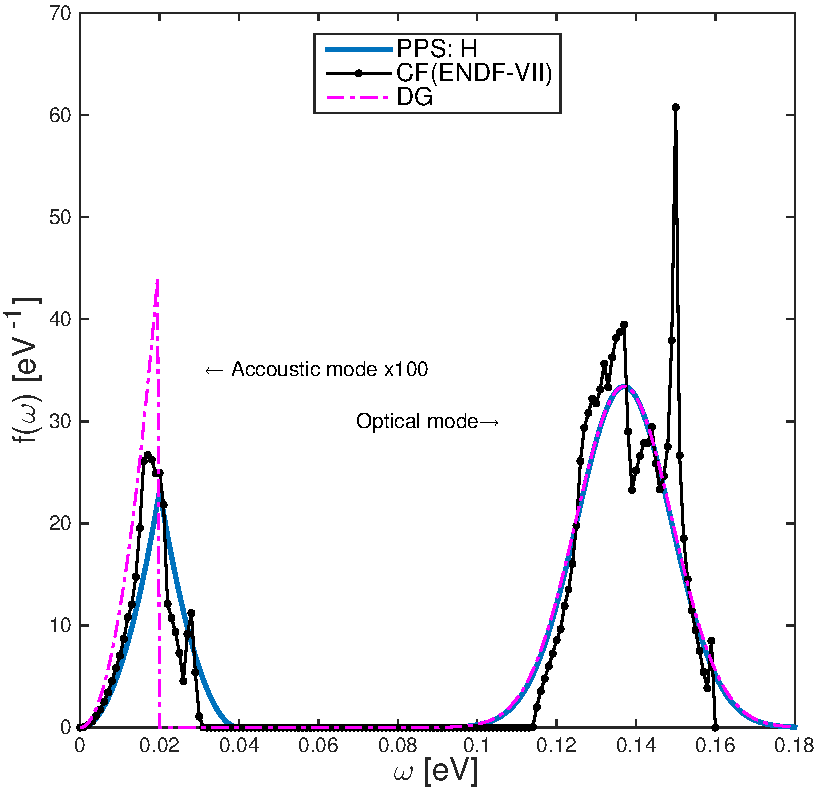
\includegraphics[width=1.4\linewidth]{NSE15-48R1_Figure1a.pdf}
		\caption{Phonon spectra of H in \zh~from CF(ENDF-VII), DG and PPS}
		\label{fg:pph1}
	\end{subfigure}
	~
	\begin{subfigure}{0.5\textwidth}
		\centering
		\hspace*{-.5cm}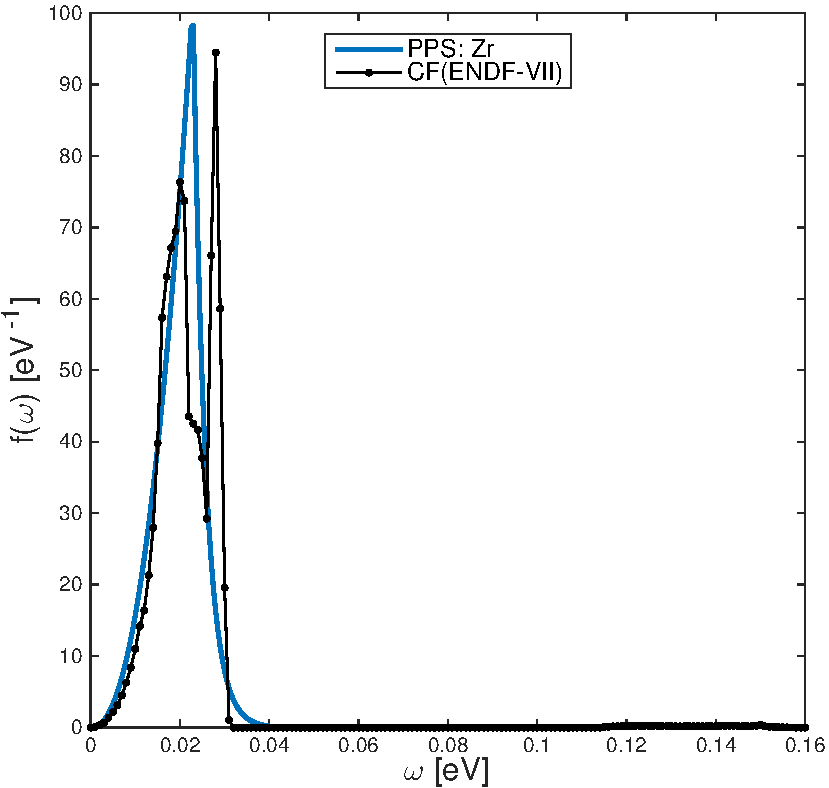
\includegraphics[width=1.4\linewidth]{NSE15-48R1_Figure1b.pdf}
		\caption{Phonon spectra of H in \zh~from CF(ENDF-VII),  and PPS}
		\label{fg:ppz1}
	\end{subfigure}
	\caption{Phonon spectrum examples. Note that Zr spectrum in DG is not plotted. It is treated as free gas, which has a spectrum of Dirac function at $\omega=0$\ eV\cite{NJOY,Macf}.}
	\label{fg:ps0}
\end{figure}

Nevertheless, the PPS model is not limited to fitting existing phonon spectra. In fact, it enables one to vary the phonon spectra in a controlled way. Figure~\ref{fg:ps}~shows some examples of phonon spectra of \zh~with parameters sampled via Latin Hypercube sampling (LHS) designs in previous work\cite{weixiong,thesis,physor}. \tcb{LHS is a type of space-filling, stratified-sampling strategy\cite{lhs}. For a total sample size of $N$ with $M$\ variables, every dimension is divided into $N/M$\ strata. Samples are then generated from randomly selecting a stratum in each dimension and assuring that each stratum is only sampled once. Upon selecting a stratum, the variable is randomly sampled within that stratum}. \tcb{The numbers in the legends are the sequence number randomly selected in a $256$~LHS design sampling. With different sets of parameters, PPS spectra are different, e.g., in peak positions and magnitudes.}

%\tcb{ It could be seen that from Figure\ \ref{fg:ps}\ that the PPS model, developed based on DG model, gains more flexibility in changing the spectrum by simply tuning the parameters.}

\begin{figure}[ht!]
\begin{subfigure}{0.5\textwidth}
\centering
\hspace*{-3.5cm}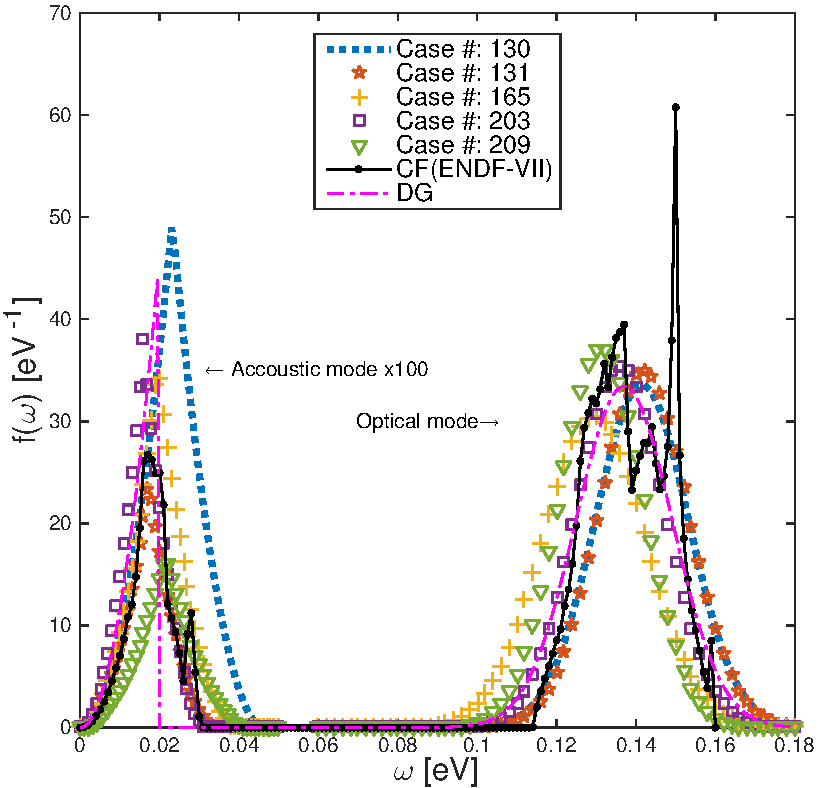
\includegraphics[width=1.4\linewidth]{NSE15-48R1_Figure2a.pdf}
\caption{Phonon spectra of H in \zh~from CF(ENDF-VII), DG and PPS}
\label{fg:pph}
\end{subfigure}
~
\begin{subfigure}{0.5\textwidth}
\centering
\hspace*{-.5cm}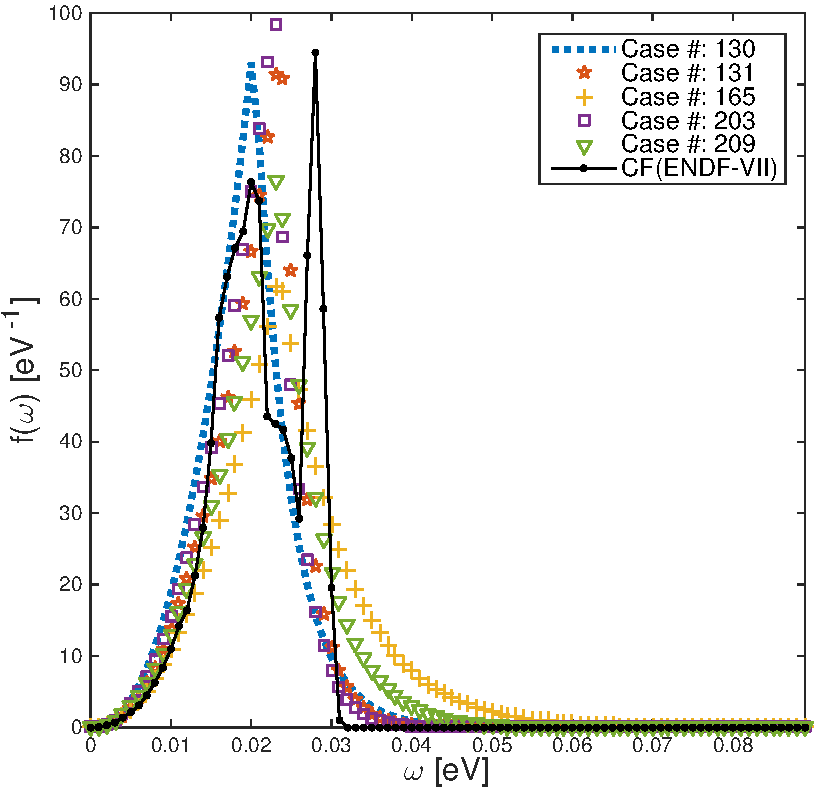
\includegraphics[width=1.4\linewidth]{NSE15-48R1_Figure2b.pdf}
\caption{Phonon spectra of H in \zh~from CF(ENDF-VII),  and PPS}
\label{fg:ppz}
\end{subfigure}
\caption{Comparisons among DG (H only), CF and PPS spectra.}
\label{fg:ps}
\end{figure}
%\footnotetext{\textcolor{blue}{(R2M9)Note that in DG model Zr is treated as free gas, which has a spectrum of Dirac function at $\omega=0$\ eV\cite{Macf,NJOY}.????????????}}

\subsubsection*{Overview of our previous work}
We uniformly sample parameters over the seven dimensional input space by using LHS designs. Picking a sample combination will produce a unique PPS defined by Eqs.~\eqref{eq:ppsh}~and~\eqref{eq:ppsz},~and finally, a unique set of scattering data.

Initially, we employed LHS to produce $3000$~samples of parameter combinations, used NJOY\cite{NJOY}\ to generate MCNP-compatible thermal data and invoked MCNP\cite{mcnp}\ to do the criticality calculations on a TRIGA lattice geometry\cite{weixiong,thesis}. A method combining \tcb{analysis of variance (ANOVA) }, with regression based cross-validation was developed to investigate the sensitivity of QoIs to parameters and the interactions between the parameters. \tcb{ANOVA is a collection of statistical tests for heterogeneity of the means of  outcomes by analyzing the variations of the response to each variable in a set of independent variables\cite{mathematica,msa,santner2003design}. A polynomial regression with the significant parameters selected in ANOVA analysis was performed to demonstrate the efficacy of the selection\cite{santner2003design}}. The reactivity $\rho$~was  found to be sensitive to the $b$~and $p$ parameters and  relatively insensitive to the others mentioned in Eq.~\eqref{eq:ppsh}.~We refer to $b$ and $p$ as the two ``main parameters".

We extended the analysis to full-core TRIGA geometry with a new and effective sampling strategy using \tcb{256 samples} which separately sampled the two parameters independently of the other five parameters\cite{physor}. {In detail, we build one sampling design on the 2-dimensional $b-p$\ space and the other design on the 5-dimensional space of the remaining parameters. The idea of this type of split-sampling is simple: we densely sample the sensitive parameters and sample the insensitive parameters in a sparse manner.}

From the full core model we found the mean neutron generation time $\Lambda$~and fuel temperature coefficient $\alpha$,~in addition to the reactivity, to be sensitive to the \tcb{main} parameters. Furthermore, we ran simulations with ENDF-VII thermal scattering data of \zh~as a surrogate of experiment and we developed a method to directly calibrate proper parameter sets to match experimental results, which will be discussed in following sections. {Though ENDF-VII only has the data for ZrH$_2$\cite{NJOY,Macf},\ the framework is not limited to ZrH$_2$: it is applicable to calibration of any type of \zh\ or thermal scattering laws for other materials.}

In this paper, we develop the calibration framework with emulators. The need for a new calibration framework is demonstrated by the fact, shown below, that to do a thorough calibration one either needs a large number of simulation results{to avoid gaps in the possible calibration result caused by lack of sample realizations in some regions of input space}. {To accomplish emulator-based calibration, Bayesian multivariate adaptive regression splines (BMARS) and Gaussian process regression (GPR) are introduced to use inputs and corresponding simulation outputs to produce regression models and predict on modeler-defined parameter mesh points.} Then we calibrate the parameters with both the {direct} calibration method and emulation based methods, predictions of which are informed by probability distributions and calibrate the parameters. We then test the calibrated parameters.
%
%\paragraph{Installation} If the document class \emph{elsarticle} is not available on your computer, you can download and install the system package \emph{texlive-publishers} (Linux) or install the \LaTeX\ package \emph{elsarticle} using the package manager of your \TeX\ installation, which is typically \TeX\ Live or Mik\TeX.
%
%\paragraph{Usage} Once the package is properly installed, you can use the document class \emph{elsarticle} to create a manuscript. Please make sure that your manuscript follows the guidelines in the Guide for Authors of the relevant journal. It is not necessary to typeset your manuscript in exactly the same way as an article, unless you are submitting to a camera-ready copy (CRC) journal.
%
%\paragraph{Functionality} The Elsevier article class is based on the standard article class and supports almost all of the functionality of that class. In addition, it features commands and options to format the
%\begin{itemize}
%\item document style
%\item baselineskip
%\item front matter
%\item keywords and MSC codes
%\item theorems, definitions and proofs
%\item lables of enumerations
%\item citation style and labeling.
%\end{itemize}

\section{Description of the ``experiment", the simulations and the framework}
\subsection{Surrogate experiment}
We run simulations with ENDF-VII thermal data for \zh~as a surrogate of a real experiment.~The QoIs generated from the ``experimental" simulations could be treated as experimental results.

The simulations for the surrogate experiments are with the full core configuration of the TRIGA reactor at \TAMU.~The geometry, specifically the shim safety rod positions, is set to make the reactor to be near critical for a $600$~K fuel temperature.
\subsection{{Calibration framework}}
{Under the same condition as the surrogate experiment, }we ran $256$\ MCNP simulations. In addition, another $256$~runs were taken with the same geometrical configuration but a different fuel temperature at $293.6$~K to explore the temperature effects. In each criticality calculation $7.5\e{7}$~particles were used in total with which the standard deviation of the $k_\mathrm{eff}$~was  about $10$~pcm for all simulations.

The basic framework of this type of UQ work is shown in Figure~\ref{fg:fc}.~From Step~1~through~4,~the PPS parameters are sampled via an LHS design and propagated through phonon spectra synthesis and data generation to simulation results. In Step~5,~the modeler needs to calibrate plausible PPS parameter values (or value sets) {using PPS-calculated QoIs generated in Step~4 with surrogate QoIs based on ENDF data}.~For this work, we also have one more step for testing the calibrated PPS parameters. The expectation is that with the calibrated parameters, we should replicate experimental results.

\begin{figure}[ht!]
  \begin{center}
    \hspace*{-1.2cm}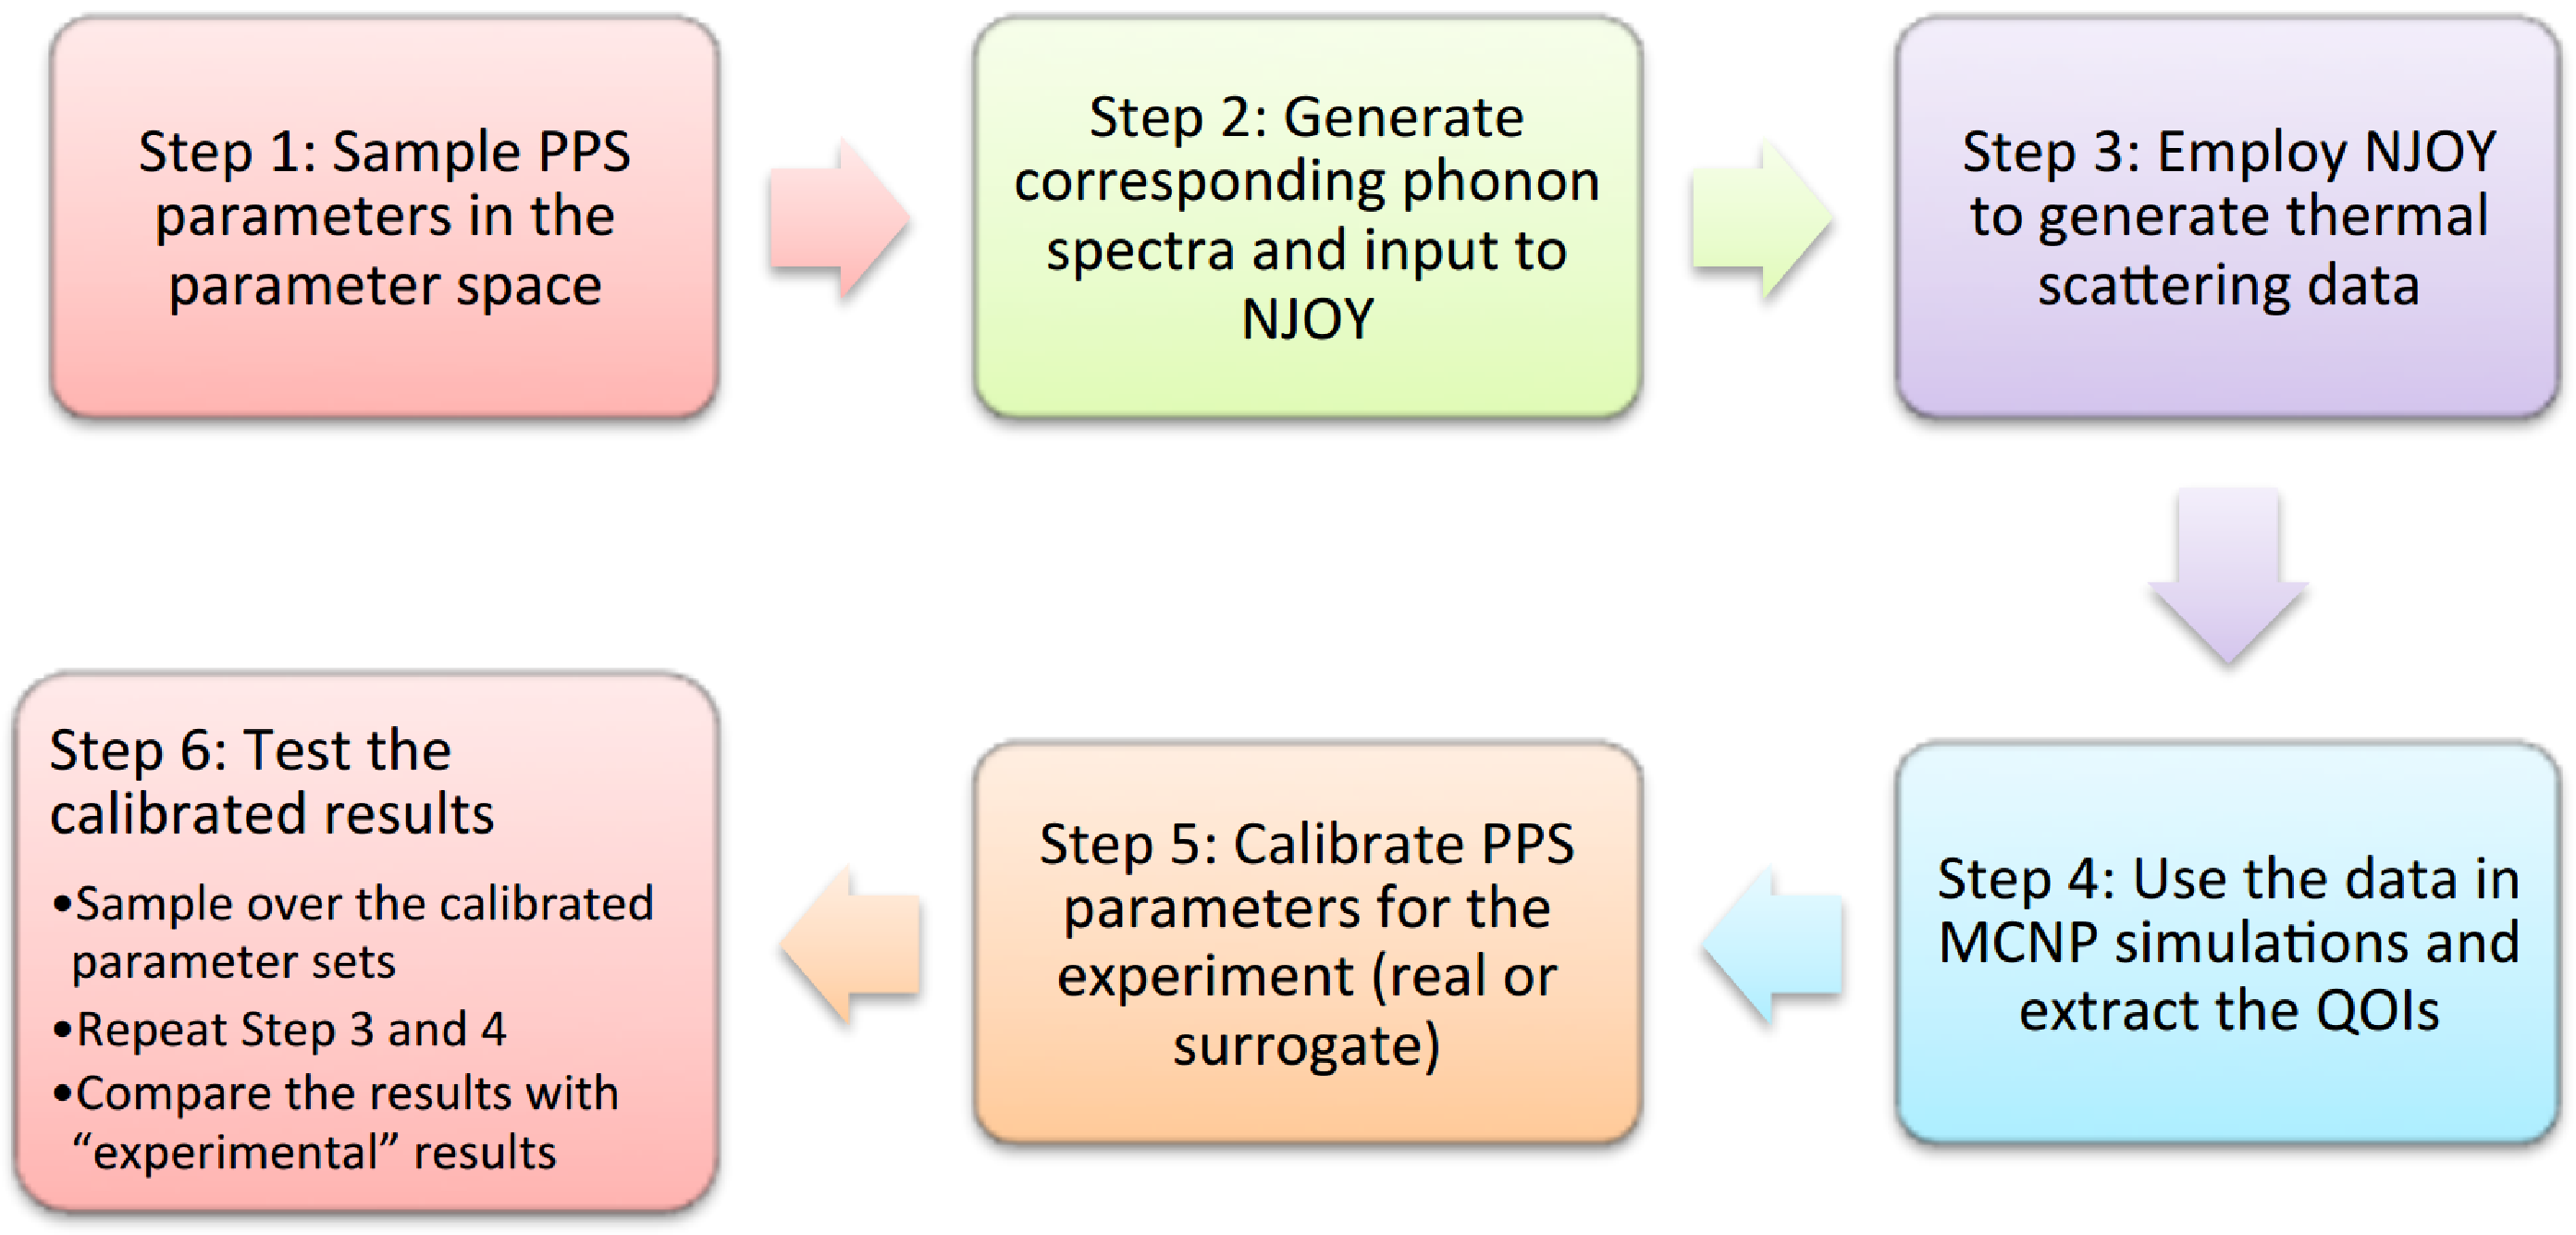
\includegraphics[width=1.2\textwidth]{NSE15-48R1_Figure3.pdf}
    %\includegraphics[width=0.45\textwidth]{srholam.eps}
    \caption[]{\label{fg:fc}The flow chart of calibration framework.}% Only the ``Figure" label and figure number are bold.}
  \end{center}
\end{figure}

In this article, we introduce several calibration techniques applied in Step~5. The performances of the techniques will be compared and shown in the following sections.

%Previous work indicates that the reactivity $\rho$,~the neutron mean generation time $\Lambda$~and the fuel temperature coefficient $\alpha$~are sensitive to parameter variations.(cite physor and ans?) 
\subsection{Sampling of parameters}
Sampling of parameters, including uncalibrated and calibrated, are sampled via LHS design. However, in our case, sampling over seven parameters with one single equal weight would not be economical since each parameter has a distinct significance. An improved sampling strategy is to base the sampling strategy on the significances of the parameters. Fortunately, in previous work, it has been revealed that only two parameters significantly affect the QoIs. Therefore we sample the significant two parameters separated from the other five through two LHS designs. One example of a design matrix of sampling 50 realizations using  two LHS designs are shown in Figure~\ref{lhsmatrix}. In this figure below the diagonal we show a 2-D projection of the samples of each pair of parameters. \tcb{Despite the fact that we sample the important parameters ($b$\ and $p$)\ more densely, the sample distributions for the other five are still appear uniform.} The diagonal shows the histogram of each parameter.\tcb{The magnitude of all bins in each histogram are almost equal, indicating the 1D projection of the sampling of each parameters is almost uniform on its own axis despite the samples are generated in multi-dimensional spaces.} Above the diagonal we print the pair-wise correlation coefficients for each pair of parameters. \tcb{Since all the absolute values of correlation coefficients are smaller than $0.3$,\ the correlations can be considered small such that each parameter is sampled independently\cite{cohen}}. %Despite the sampling is biased, the realizations in each dimension are still roughly uniformly distributed. Specifically,
%Specifically, the LHS design matrix of the two main parameters is shown in Figure~\ref{lhsmain}.\ \tcb{Graphically it presents a uniform distribution in the 2D parameter space.}

\begin{figure}[ht!]
	\begin{center}
		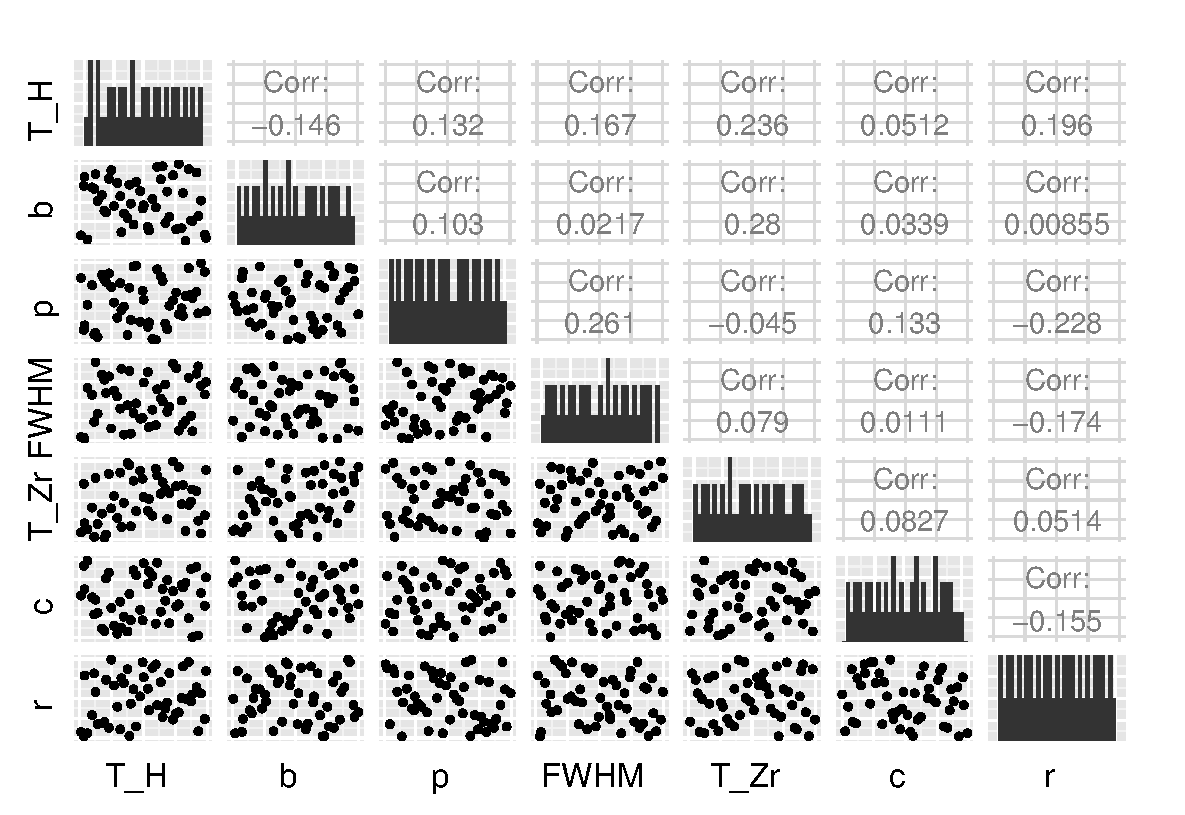
\includegraphics[width=1.\textwidth]{NSE15-48R1_Figure4.pdf}
		%\includegraphics[width=0.45\textwidth]{srholam.eps}
		\caption[]{\label{lhsmatrix}LHS design matrix with 50 samples.}% Only the ``Figure" label and figure number are bold.}
	\end{center}
\end{figure}

%\begin{figure}[ht!]
%	\begin{center}
%		\includegraphics[width=1.\textwidth]{lhsmain.eps}
%		%\includegraphics[width=0.45\textwidth]{srholam.eps}
%		\caption[]{\label{lhsmain}LHS design matrix for the main parameters with 50 samples.}% Only the ``Figure" label and figure number are bold.}
%	\end{center}
%\end{figure}

\section{Direct calibration}
One could accomplish the goal of calibration via measuring how close the simulation results (outputs) are to the target or experimental results and collecting parameter sets with which one could construct phonon spectra and generate scattering data to make the simulation results close to the experiment. We name the measure process ``scoring". {The scoring process requires a quantitative measure of agreement between simulation and experiment. MCNP generates QoIs as normal distributions with an estimated mean and standard deviation. Assuming the experimental results are also given in this form\footnote{Surrogate experiments performed in MCNP naturally suit this assumption.}, then the score could be defined as the overlap between realization and measured normal distributions, as the example illustrated in Figure~\ref{fg:score}.~In the example, two Gaussian distributions intersect with each other and the shadow  is the overlap. We, thereafter, analytically compute the overlap for all realization of simulations to archive the scores and project the scores into the PPS parameter space. The ``spatial" distribution of the scores in the parameter space indicates parameters that give good agreement with the target output. The simulation results are made with scattering data based on the phonon spectra constructed with the PPS parameters.} The expectation is that the collection from all high-score realizations could form a subset of parameters in the parameter space such that simulation with \zh~thermal scattering data generated with those parameter subsets would be accurate compared with the measured or experimental results.

\begin{figure}[ht!]
  \begin{center}
    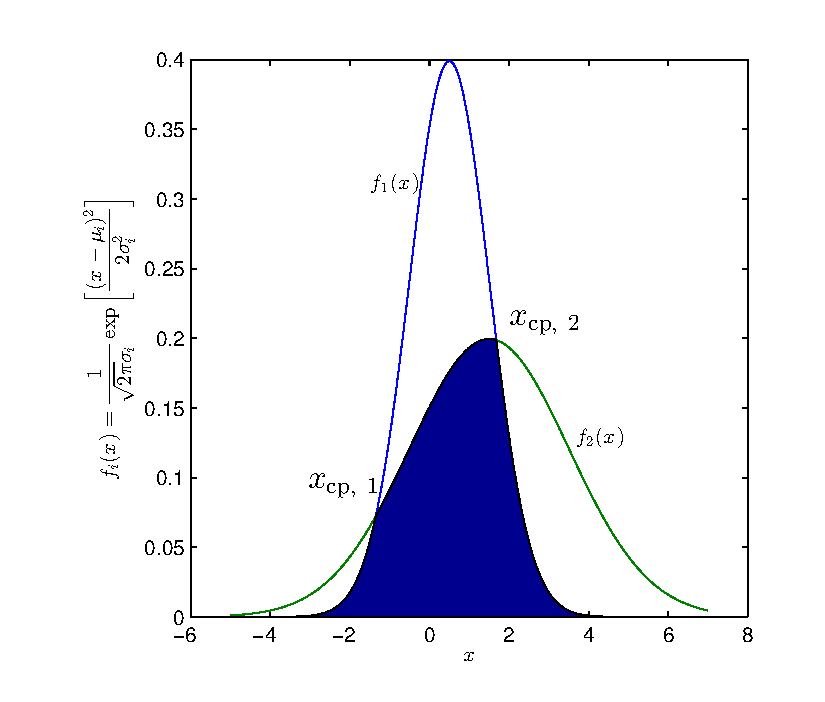
\includegraphics[width=0.67\textwidth]{NSE15-48R1_Figure5.pdf}
    %\includegraphics[width=0.45\textwidth]{srholam.eps}
    \caption[]{\label{fg:score}Example of the score estimation.}% Only the ``Figure" label and figure number are bold.}
  \end{center}
\end{figure}

 %Figure.~xxx (srho needed) is an example of projecting the scores with 

For each type of QoI, we can estimate the distribution of the scores once. Figure~\ref{fg:narrow}~is the example of scoring with the reactivity $\rho$.~Since previous studies \cite{weixiong,physor} showed only $b$, the branching ratio of acoustic mode of H in \zh,~and $p$,~the peak position of optical mode of H,~to be the sensitive parameters, in this study all calibrations focus on these two parameters and the scores are only projected into the $b$-$p$~2D parameter space\footnote{Interested readers may refer to Ref.~\cite{santner2003design} for a more detailed explanation of this process. The physical significance of these two parameters can be explained as follows. Slaggie's solid mechanics model is based on four constants describing four types of inter-atomic interactions in \zh\ molecules\cite{Slaggie}. It indicates that changing the constant that describes the Zr-Zr interactions would cause the change in the acoustic mode magnitude, or equivalently, the branching ratio $b$. Conversely, changing $b$\ can have the same effect as changing the impact from Zr-Zr interactions in the solid. The $p$\ parameter represents the excitation state of the optical mode. It can be realized that, varying the excitation state of the optical mode of H in \zh\ would cause changes in the scattering with the low-energy neutrons.} 

Moreover, when scoring with multiple types of QoIs simultaneously, the multiplication of the score distributions  narrows the size of the parameter subset. Figure~\ref{fg:narrow3}~is made with scoring with $\rho$,~$\Lambda$~and $\alpha$,~which shows the most likely values of $b$~and $p$~reproducing the surrogate experiment plausibly. In theses results most likely appropriate $b$~is about $0.01$~and $p$~is about $137$~meV.

\begin{figure}[ht!]
\begin{subfigure}{0.5\textwidth}
\centering
\hspace*{-1.5cm}
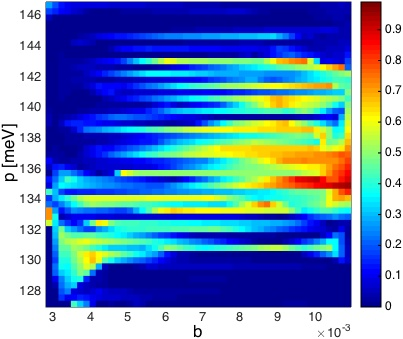
\includegraphics[width=1.2\linewidth]{NSE15-48R1_Figure6a.jpg}
\caption{Calibration example with ENDF-VII projected onto the main-parameter subspace. QoI: $\rho$.}
\label{fg:narrow}
\end{subfigure}
~
\begin{subfigure}{0.5\textwidth}
\centering
\vspace*{.7cm}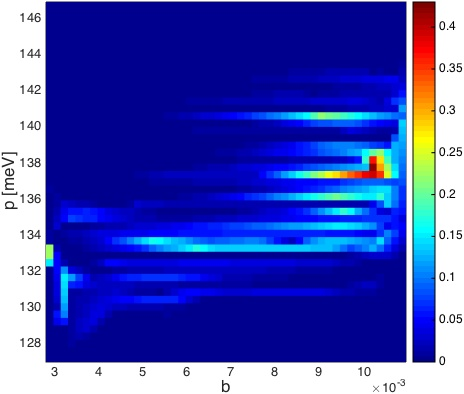
\includegraphics[width=1.2\linewidth]{NSE15-48R1_Figure6b.jpg}
\caption{Calibration example with ENDF-VII projected onto the main-parameter subspace. Scores are from the multiplication of scores for $\rho$,~$\Lambda$~and $\alpha$.}
\label{fg:narrow3}
\end{subfigure}
\caption{Calibration with multiple QoIs.}
\label{fig:cb}
\end{figure}

%%%%%%%%%%%%%%%%%%%%%%%%%%%%%%%%%%%%%%%%%%%%%%%%%%%%%%%%%%%%%%%%%%%%%%%%%%%%%%%%%%%%%%%%%%%%%%%%%%%%%%%%%%%%%%
\section{Emulation-based calibration}
The direct calibration succeeds in finding preferred parameter subsets as illustrated in Figure~\ref{fig:cb}.~However, due to the sparseness of the calibrated results caused by the relatively small size of samples ($256$),~it has the drawback that {there exist gaps in the calibrated parameter scores.} This creates an irregularly-shaped high-score region that is imprinted with the set of samples from parameter space.  
The intuitive way to avoid or mitigate the data gaps would be to increase the sample numbers of the parameter combinations and generate many sets of scattering data to run MCNP simulations and gain smoother and more continuous score distributions. Nevertheless, the computational expense could be insurmountable to reach this goal. Therefore, it is reasonable to develop methods to {effectively perform the calibration without necessitating a dense sampling of the input space}. The methods should be able to give smooth score distributions when appropriate and must be computationally affordable.

One posisble approach is to create a map from the inputs to the outputs from limited numbers of simulations. Assuming the inputs $X$~and simulation outputs $Y_\mathrm{i}$, where the subscript $i$ denotes a QoI, are subject to relationships hidden in the code (e.g.~MCNP in this case), we want to establish a  model for the mapping $f:X\mapsto R$ such that
\begin{equation}\label{eq:fitmodel}
Y_\mathrm{i}=f(X)+\epsilon_\mathrm{i},~X\in D,
\end{equation}
where $\epsilon_\mathrm{i}$~is a random error and $D$~is the input parameter space.  Such a model is sometimes called an emulator or, alternatively, a surrogate model.
Moreover, given inputs, we also expect the emulators to generate outputs informed by probabilistic distributions representing the confidence in the results, with which we could apply the scoring strategy developed for direct calibration. Some Bayesian inferred emulators hold these properties. Candidates in this work are Gaussian process regression (GPR) and Bayesian multivariate adaptive regression splines (BMARS) inspired by the their performances in radiation-hydrodynamics experiments in McClarren~et al's work\cite{pie},~among others.
\subsection{Gaussian process regression}
Gaussian process regression generates distributions of functions (emulation outputs) which interpolate the output data in the training dataset. A Gaussian process (GP) is a collection of random variables. Any subsets of such collection has a joint Gaussian distribution. GP defines the mapping (the regression model) from the inputs to the outputs, i.e.~$f:X\mapsto R$,~to be fully specified by a mean function $\mu(X)$~and a covariance function $k(X,X')$ (also called ``kernel"):
\begin{equation}
f(X)\sim \mathcal{GP}(\mu(X),k(X,X')),
\end{equation}
\tcb{where $f(X)$\ is the function value at location $X$\ in the input space and the covariance function $k$\ specifies the covariance between the pair of random variables $(X,\ X')$\ in the input space.}

And it is often assumed that
the error is subject to a normal distribution with user-defined variance $\sigma_\mathrm{n}^2$:
\begin{equation}
\epsilon_\mathrm{i}\sim N(0,\sigma_\mathrm{n}^2),
\end{equation}
therefore $Y_\mathrm{i}$~in Eq.~\eqref{eq:fitmodel}~obeys
\begin{equation}
Y_\mathrm{i}\sim GP(\mu(X),k(X,X')+\delta_{XX'}\sigma_\mathrm{n}^2),
\end{equation}
where $\delta_{XX'}$~is the Kronecker delta.
In practice, one is free to choose the type of the kernel. In this paper, we choose to use fully squared exponential kernel, shown in Eq.~\eqref{eq::covseard},~to assure smoothness of the emulation outputs \cite{pie}. This kernel is given by
\begin{equation}\label{eq::covseard}
k(X_\mathrm{i},X_\mathrm{j})=\sigma_\mathrm{f}^2\exp\left\{-\frac{1}{2}\left(X_\mathrm{i}-X_\mathrm{j}\right)^\top\left(\mathcal{D}^{-1}\right)^2\left(X_\mathrm{i}-X_\mathrm{j}\right)\right\}
\end{equation}
where the $\sigma_\mathrm{f}^2$~is the maximum value of the covariance. $\mathcal{D}$~is a diagonal parameter matrix. {It is usual to write $\theta=\{\sigma_\mathrm{f},~\sigma_\mathrm{n},~\mathcal{D}\}$~as ``hyperparameters", which would not be user-designated, but be calculated in the procedure of building the emulator\cite{carl}.}.
The parameters of the kernels are estimated in the Bayesian inference procedure (see, for instance Ref.~\cite{carl}).
Then the covariance matrix element between two different input points can be calculated as:
\begin{equation}
K_{\mathrm{ij}}=k(X_\mathrm{i},X_\mathrm{j}).
\end{equation}
One formulates the predictions contingent upon the training data by:
\begin{equation}\label{mark}
f^*|f\sim N(\mu^*+K^{*\top} K^{-1}(f-\mu),K^{**}-K^{*\top} K^{-1}K^*)
%\left[\begin{array}{c}
%f\\
%f^*
%\end{array}\right]\sim N\left(\left[\begin{array}{c}
%\mu\\\mu^*
%\end{array}\right],\left[\begin{array}{cc}
%K & K^*\\
%{K^*}^\top & K^{**}
%\end{array}\right]\right),
\end{equation}
where \tcb{the quantities $X$,~$f$,~$X^*$~and $f^*$~are the training set inputs, corresponding function values, modeler-defined input values (test input) and predictions at the input points (or point sets for multi-D cases) from GPR, respectively.  Additionally,} $K_{\mathrm{ij}}=k(X_\mathrm{i},X_\mathrm{j}),~K^*_{\mathrm{ij}}=k(X^*_\mathrm{i},X_\mathrm{j})~\mathrm{and}~K^{**}_{\mathrm{ij}}=k(X^*_\mathrm{i},X^*_\mathrm{j})$. Therefore, GPR generates a Gaussian distribution with a mean and a covariance at each points we designated for interest.

Figure~\ref{fg:gpex}~is an example of GPR emulation. The dot points are generated from a logistic function with normal errors. The GPR emulator, as observed, follows the trend of data to infer the underlying function, GPR also generates interpolated function distributions informed by normal distribution; the variance in the distribution this is used to infer the uncertainty in the fit.

\begin{figure}[ht!]
  \begin{center}
    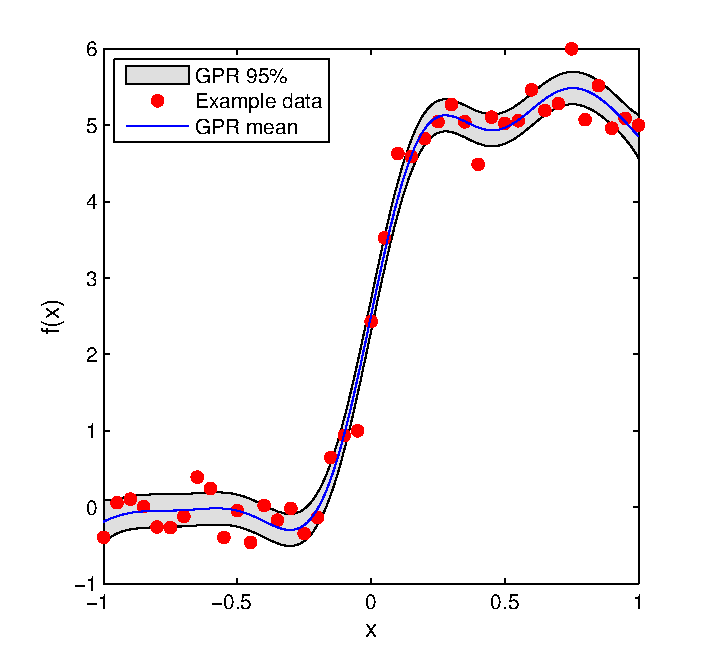
\includegraphics[width=0.7\textwidth]{NSE15-48R1_Figure7.pdf}
    %\includegraphics[width=0.45\textwidth]{srholam.eps}
    \caption[]{\label{fg:gpex}Example of GPR 1D data fitting for a logistic function.}% Only the ``Figure" label and figure number are bold.}
  \end{center}
\end{figure}


%Furthermore, the first-order interactions ($X_\mathrm{i}X_\mathrm{j}, \mathrm{i,j}=1,\cdots,7~\mathrm{and~i}\ne\mathrm{j}$)~are also tested with both methods. The significances of interactive terms are observed lower than those non-interactive terms. Another indication, which actually has been applied in this paper, is that it might be convincing to get good results with modeling with only non-interactive terms. This idea reduce the modeling dimensionality. Actually, we have already proved with polynomial regression that this type of dimension reduction actually helped improve the accuracy of the prediction\cite{thesis}.(cite my thesis and physor) As an example Figure~\ref{fg:rho_all}~and \ref{fg:rho_non}~show the GPR emulated reactivity $\rho$~with fuel temperature of $293.6$~K with all terms including interactions and only seven non-interactive terms, respectively. One might not tell the difference between the these two sets of emulation results. Specifically, Figure~\ref{fg:modelcomp}~shows the comparisons between these two sets. Actually, the largest difference is smaller than $0.5$~\%.\textcolor{blue}{Any drawback of using complex regression model over simple model?}

%\begin{figure}[ht!]
%\begin{subfigure}{0.31\textwidth}
%\centering
%\includegraphics[width=0.9\linewidth]{gpr_rho_all.eps}
%\caption{GPR emulated $\rho$~with non-interactions and interactions vs simulations.}
%\label{fg:rho_all}
%\end{subfigure}
%~
%\begin{subfigure}{0.31\textwidth}
%\centering
%\includegraphics[width=0.9\linewidth]{gpr_rho_non.eps}
%\caption{GPR emulated $\rho$~with non-interactions vs simulations.}
%\label{fg:rho_non}
%\end{subfigure}
%~
%\begin{subfigure}{0.31\textwidth}
%\centering
%\includegraphics[width=0.9\linewidth]{gpr_mod_com.eps}
%\caption{Comparison between results from two models.}
%\label{fg:modelcomp}
%\end{subfigure}
%\caption{Results comparison between different GPR models.}
%\label{fg:gprmodel}
%\end{figure}



\subsection{Bayesian Multivariate Adaptive Regression Splines (BMARS)}
For this paper, we choose BMARS as a candidate emulator as well as GPR.  BMARS arose originally from multivariate adaptive regression splines (MARS) developed by Friedman\cite{friedman1991}. MARS is a curve-fitting technique which emulates the relationship between the inputs and outputs as a summation of spline functions at different orders\cite{stripbmars}. In the 1D case, the spline functions are defined to be continuous and polynomial functions at some order on part of the domain and zero otherwise. Multivariate splines are simply multiplications of 1D spline functions. MARS linearly combines those splines to construct bases functions. Following the same notations in Ref.~\cite{pie},~Eq.~\eqref{eq::basis}~shows an example of basis function:
\begin{equation}\label{eq::basis}
B_\mathrm{i}(X)=
\begin{cases}
1 & \mathrm{i}=0\\
\prod\limits_{\mathrm{j}=1}^{\mathrm{J_i}}\left[s_{\mathrm{i,j}}(X_{\mathrm{v(i,j)}}-t_{\mathrm{i,j}})^{r_\mathrm{i}}\right]_+ & \mathrm{i}=1,2,...
\end{cases}
\end{equation}
where $X$~is the input matrix, each column of which is an input parameter vector or the interaction of two input vectors,  $(\cdot)_+\equiv\max \{0,\cdot \}$, and ~$t_\mathrm{i,j}$~is a knot point. With the $(\cdot)_+$~operator, the splines has nonzero values when the inputs are larger than the knot values. $r_\mathrm{i}$~is the order of the spline function. Index $\mathrm{v(i,j)}$~gives the split on knot $t_{\mathrm{i,j}}$; $s_{\mathrm{i,j}}$~is the sign indicator.

Then with those basis functions, the MARS estimated $f$~can be expressed by:
\begin{equation}
f(X)=\sum\limits_{\mathrm{i}=0}^{\mathrm{I}}\beta_\mathrm{i}B_\mathrm{i}(X),
\end{equation}
where $\beta_\mathrm{i}$\ is the coefficient or weight associated with the $\mathrm{i^{th}}$\ basis function $B_\mathrm{i}(X)$\cite{bmars_mcc2,stripbmars}.

Denison et al.~introduced Bayesian  MARS (BMARS) that generates a posterior distribution of predictive MARS function\cite{malick}. The estimations of making inference of the posterior predictive distributions involves a Markov chain Monte Carlo process (MCMC).

Figure~\ref{fg:bmex1}~shows several predictions sampled from posterior distributions. And Figure~\ref{fg:bmex2} is the example of prediction data with $95$~\% confidence interval. It is noted that BMARS results in distributions asymmetric about the mean prediction. Although both BMARS and GPR interpolate functions with distributions, BMARS generate finite samples of the interpolants, while GPR has a continuous functional form for the distribution. This implies one does not get a simple expression for the predictions for each input set.

\begin{figure}[ht!]
\begin{subfigure}{0.5\textwidth}
\centering
\hspace*{-2.2cm}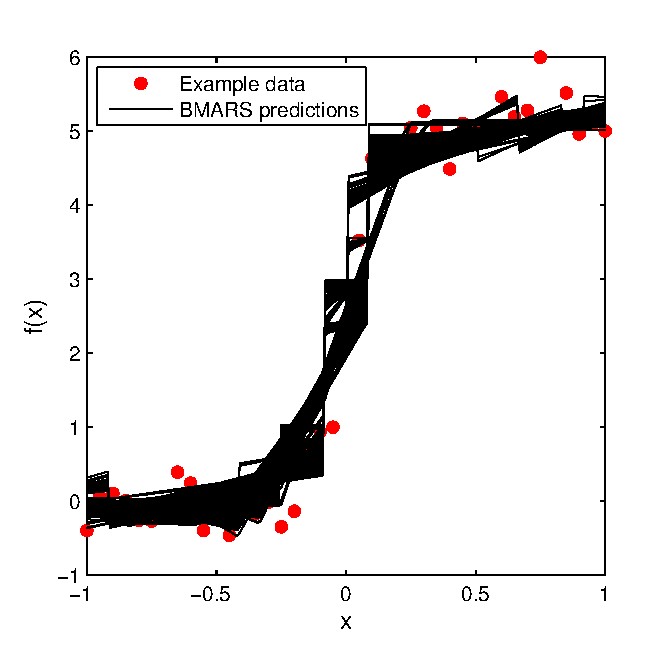
\includegraphics[width=1.4\linewidth]{NSE15-48R1_Figure8a.pdf}
\caption{Example of BMARS 1D data fitting. The regression models are drawn in MCMC procedure when inferring.}
\label{fg:bmex1}
\end{subfigure}
~
\begin{subfigure}{0.5\textwidth}
\centering
\vspace*{-0.5cm}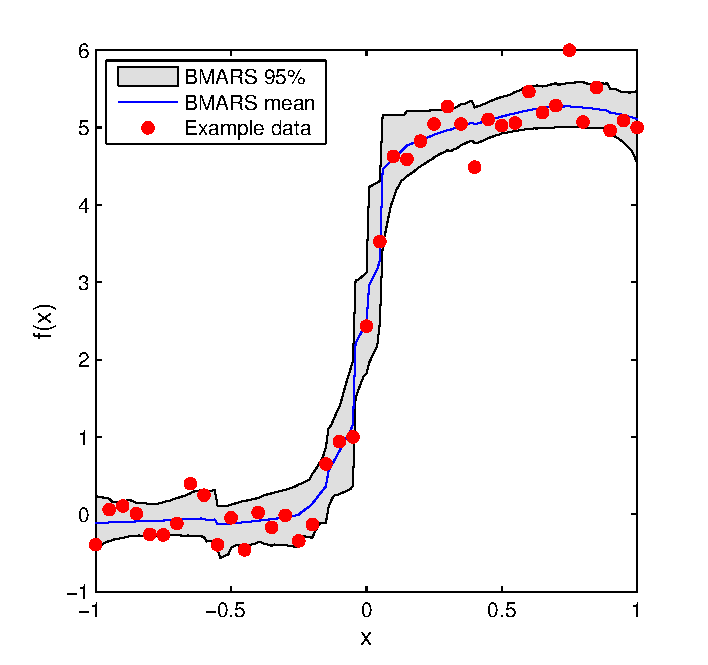
\includegraphics[width=1.4\linewidth]{NSE15-48R1_Figure8b.pdf}
\caption{Example of BMARS 1D data fitting (with $95$~\% confidence interval).}
\label{fg:bmex2}
\end{subfigure}
\caption{Example of BMARS 1D data fitting for the logistic function.}
\label{fg:bmexs}
\end{figure}


%\begin{figure}[ht!]
%  \begin{center}
%    \includegraphics[width=0.7\textwidth]{bmex1.eps}
%    %\includegraphics[width=0.45\textwidth]{srholam.eps}
%    \caption[]{\label{fg:bmex1}Example of BMARS 1D data fitting. The regression models are drawn in MCMC procedure when inferring.}% Only the ``Figure" label and figure number are bold.}
%  \end{center}
%\end{figure}
%
%\begin{figure}[ht!]
%  \begin{center}
%    \includegraphics[width=0.7\textwidth]{bmex2.eps}
%    %\includegraphics[width=0.45\textwidth]{srholam.eps}
%    \caption[]{\label{fg:bmex2}Example of BMARS 1D data fitting (with $95$~\% confidence interval).}% Only the ``Figure" label and figure number are bold.}
%  \end{center}
%\end{figure}
\subsection{Emulation based calibration}
The application of emulators in calibration would not change the protocol described in Figure~\ref{fg:fc}. The only change is the method we apply in Step~5~for calibration. Instead of direct calibration, we train the emulators with simulation results to gain a mapping from the inputs to the outputs. With modeler defined inputs, emulators generate predictive outputs from a mapping. Then, we can score the emulated results and project them onto the defined input parameter meshes and find the desired calibrated parameter sets.
\subsection{Calibration implementation}
Since GPR generates predictions given by a normal distribution, fortunately, the scoring algorithm developed for direct calibration could directly be applied to GPR emulated results (see Figure~\ref{fg:score}).

However, BMARS emulated results, which are not subject to normal distributions, disable the application of the original scoring strategy. This drives us to develop an alternative method. Since BMARS generate a set of samples from distributions as shown in Figure~\ref{fg:score},~somewhat similar with GPR's distributed results, it is natural to come up with generating an discrete probability distribution (histogram) with those samples and then calculating the overlap between each realized output and the experimental or measured distribution. Figure~\ref{fg:bmarsscore}~is an example for scoring in such way. One of the benefits is that the modeler does not need to know the analytical form of the emulation distribution. The BMARS emulation results do not need to be assumed as Gaussian, which does not necessarily hold. %\footnote{Such assumption would be wrong, though, it actually worked quite well as a compromise of using original scoring algorithm in the first trial of BMARS.}
\begin{figure}[ht!]
  \begin{center}
    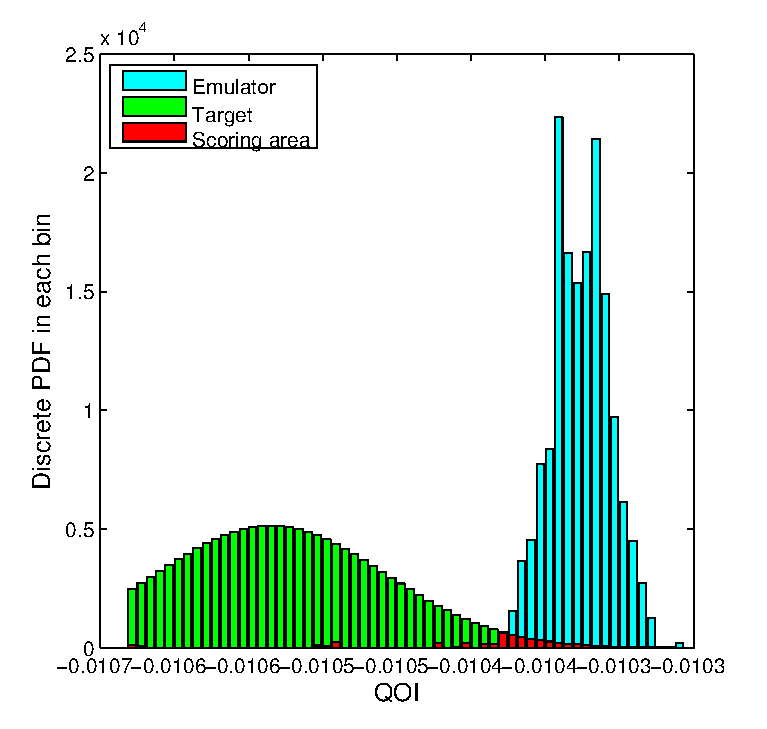
\includegraphics[width=1\textwidth]{NSE15-48R1_Figure9.pdf}
    %\includegraphics[width=0.45\textwidth]{srholam.eps}
    \caption[]{\label{fg:bmarsscore}Scoring example with BMARS emulated QoI.}% Only the ``Figure" label and figure number are bold.}
  \end{center}
\end{figure}


\subsection{GPR based calibration results}
\subsubsection{Significant parameter selection}
As stated earlier, not all seven parameters are necessarily needed to gain plausible models fitting the simulation data. To rule out the insignificant members, several techniques could be employed. %One of them could be ANOVA. Also, 
GPR has the capability of testing the significance of inputs to outputs\cite{pie}. The diagonals of $\Lambda$~are the characteristic length scales, which measure the responsiveness of outputs to input vectors if inputs and outputs are standardized before modeling.\footnote{Denote the standard deviation and mean of random variable $X$~by $\sigma$~and $\mu$, respectively, then the standardized form of $X$~is $\hat{X}\equiv\frac{X-\mu}{\sigma}$. The standardization of variables enables one to measure different variables in the same scale.} With such standardized inputs and outputs, the reciprocals of scale lengths of matrix $\Lambda$~measures the significances of corresponding input parameters\footnote{McClarren et al.~used ``relative relevance" for the diagonal reciprocal, we continue to use the same terminology in this paper}\cite{pie}. As an example. Figure~\ref{fg:sigs}~show the comparison between the GPR informed significances (relative relevance) and ANOVA informed significances (mean sums of the squares) of the parameters on reactivity $\rho$.~$X_\mathrm{1}$~through $X_\mathrm{7}$~denotes the standardized forms of FWHM,~$b$,~$p$,~$T_\mathrm{H}$,~$T_\mathrm{Zr}$,~$r$~and $c$,~respectively. Basically, both results show $b$~and $p$~(which are $X_\mathrm{2}$~and $X_\mathrm{3}$,~respectively.) are the most important two parameters, especially $p$~($X_\mathrm{3}$).

\begin{figure}[ht!]
\begin{subfigure}{0.5\textwidth}
\centering
\hspace*{-2.3cm}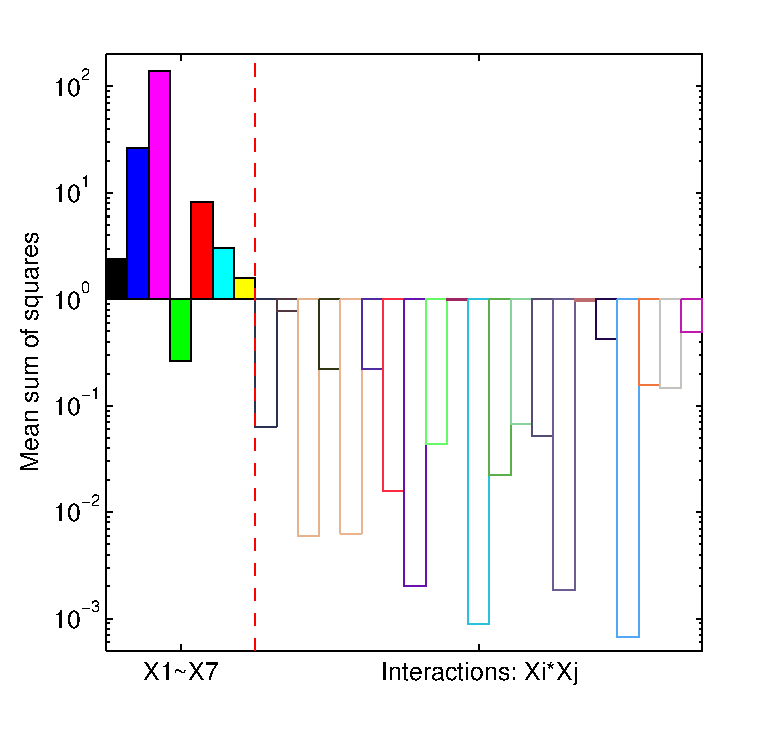
\includegraphics[width=1.4\linewidth]{NSE15-48R1_Figure10a.pdf}
\caption{Parameter significances (mean sums of squares) from ANOVA analysis.}
\label{fg:anova_sig}
\end{subfigure}
~
\begin{subfigure}{0.5\textwidth}
\centering
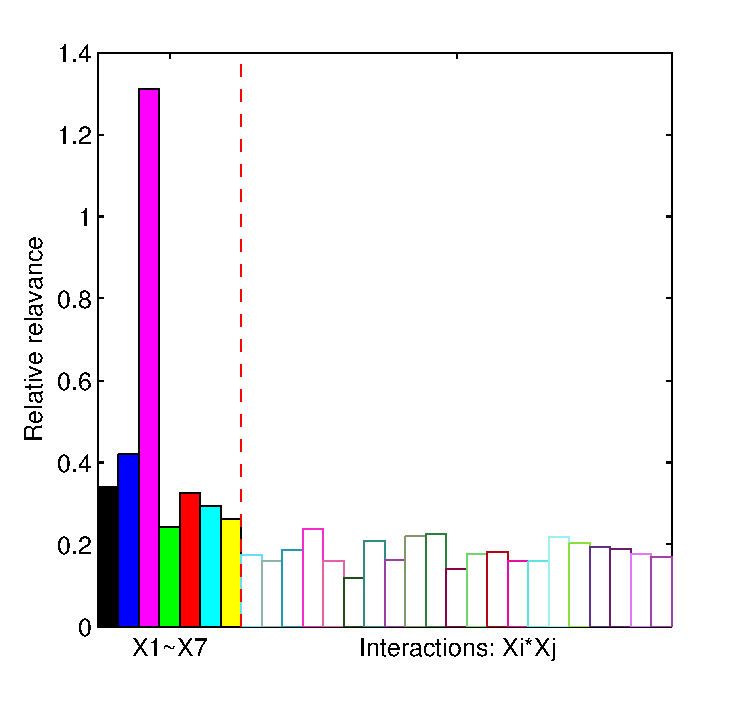
\includegraphics[width=1.4\linewidth]{NSE15-48R1_Figure10b.pdf}
\caption{Parameter significances (relative relevance) from GPR emulation.}
\label{fg:gpr_sig}
\end{subfigure}
\caption{Parameter significance comparisons from different methods.}
\label{fg:sigs}
\end{figure}

Another possible way of performing significance discrimination is to score based on emulations with all seven parameters. The score measures relative significance of the parameters. Projecting the scores into the parameter space would reveal the sensitivity of the QoIs to parameters qualitatively and clearly. Score distribution would form preferences in the subset of significant inputs and give a uniform calibrated distribution for an insignificant parameter. An example is the calibration with all seven parameters. The scores are projected on 2D parameter planes as illustrated in Figure~\ref{gp7}.~Apparently, the high score regions of $p$,~the H optical mode peak, are always strictly limited, while for other parameters other than $b$,~the H acoustic mode branching ratio, the high scores spread uniformly over the possible ranges. In other words, for parameters other than $p$~and $b$,~randomly picking a value in the parameter's range would not result in significant change in simulation results. Specifically for $b$ in Figure~\ref{gp23},~the high score region jointly distributes showing the dependence on both $b$~and $p$, which actually demonstrate the results from ANOVA and shrink our input parameter space from 7~to 2.

\begin{figure}[ht!]
\begin{subfigure}{0.5\textwidth}
\centering
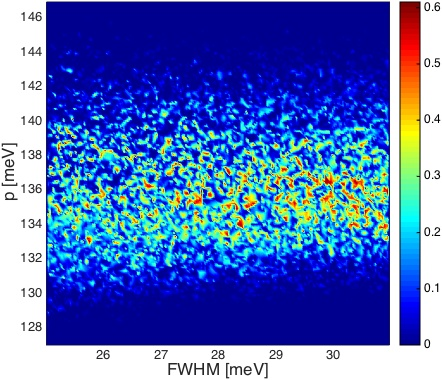
\includegraphics[width=0.9\linewidth]{NSE15-48R1_Figure11a.jpg}
\caption{FWHM$-p$~plane.}
\end{subfigure}
~
\begin{subfigure}{0.5\textwidth}
\centering
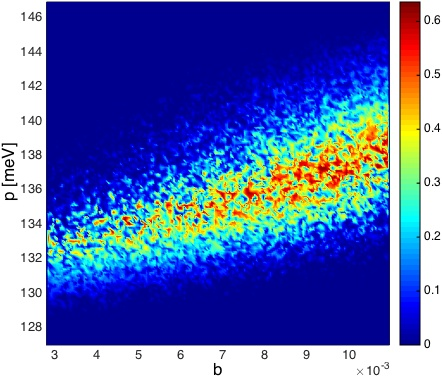
\includegraphics[width=0.9\linewidth]{NSE15-48R1_Figure11b.jpg}
\caption{$b-p$~plane.}
\label{gp23}
\end{subfigure}\\

\begin{subfigure}{0.5\textwidth}
\centering
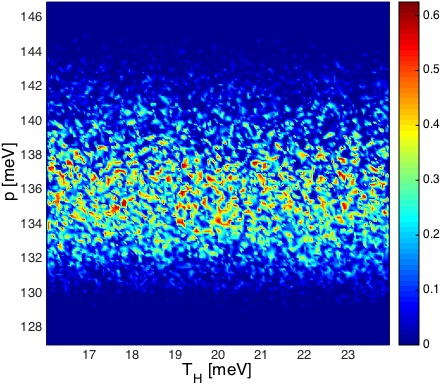
\includegraphics[width=0.9\linewidth]{NSE15-48R1_Figure11c.jpg}
\caption{$T_\mathrm{H}-p$~plane.}
\end{subfigure}
~
\begin{subfigure}{0.5\textwidth}
\centering
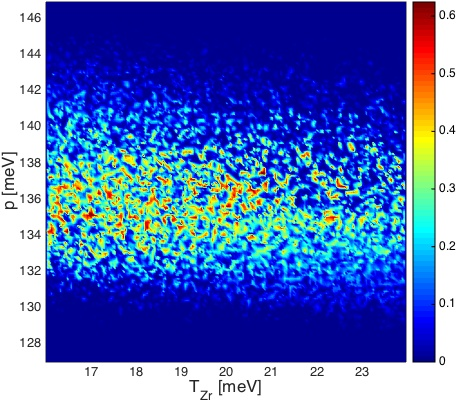
\includegraphics[width=0.9\linewidth]{NSE15-48R1_Figure11d.jpg}
\caption{$T_\mathrm{Zr}-p$~plane.}
\end{subfigure}\\

\begin{subfigure}{0.5\textwidth}
\centering
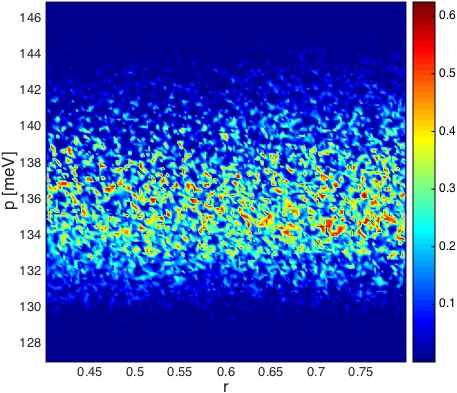
\includegraphics[width=0.9\linewidth]{NSE15-48R1_Figure11e.jpg}
\caption{$r-p$~plane.}
\end{subfigure}
~
\begin{subfigure}{0.5\textwidth}
\centering
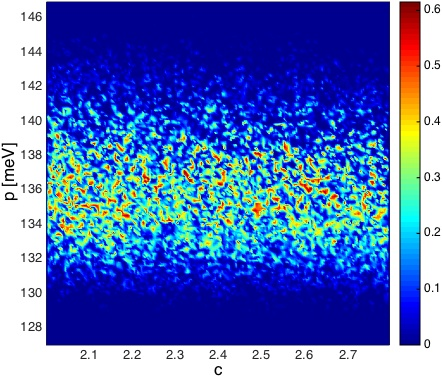
\includegraphics[width=0.9\linewidth]{NSE15-48R1_Figure11f.jpg}
\caption{$c-p$~plane.}
\end{subfigure}
\caption{The scores from GPR-based calibration with 7 parameters projected onto two-dimensional planes.}
\label{gp7}
\end{figure}


\subsubsection{GPR based significant parameter calibrations}
Figure~\ref{fg:gprcal}~is the calibration result with GPR emulator. As expected, calibrating with emulated QoIs, with only introducing two significant parameters in the model, generate smooth and continuous scoring results. Also, the score distribution is much flatter. Nevertheless, qualitatively, the high score region remains similar to that from direct calibrations. The high scores are centered around the region with $b$~of $0.01$~and $p$~of $138$~meV, the result is consistent with direct calibration.

\begin{figure}[ht!]
  \begin{center}
    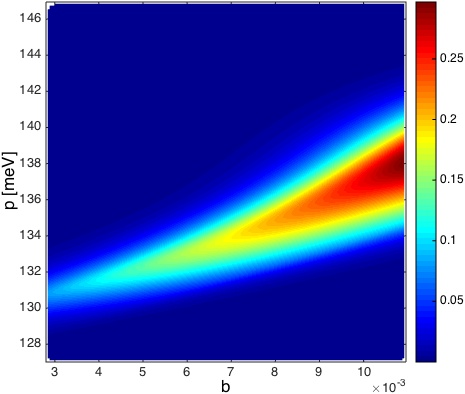
\includegraphics[width=0.7\textwidth]{NSE15-48R1_Figure12.jpg}
    %\includegraphics[width=0.45\textwidth]{srholam.eps}
    \caption[]{\label{fg:gprcal}Calibration with GPR.}% Only the ``Figure" label and figure number are bold.}
  \end{center}
\end{figure}

\subsection{BMARS based calibration results}
As the calibration results in Figure~\ref{fg:bmarscal} show, %~although the high-scored region has different shape as GPR calibrated result as the high-score region is more densely distributed, 
BMARS calibrates the parameters around the same  high-score region indicated by direct calibration and GPR. The shape of the BMARS scoring result is irregular compared with GPR. %One reasonable hypothesis based on observations is BMARS would can capture outliers forming  the irregularity.
The high scores remain near the region with $b$~of $0.011$~and $p$~of $137$~meV, differing from GPR's $p$~of $138$~meV. And though the calibrated $p$~value is close to the direct calibration result, the $b$,~however, is a little larger. 

\begin{figure}[ht!]
  \begin{center}
    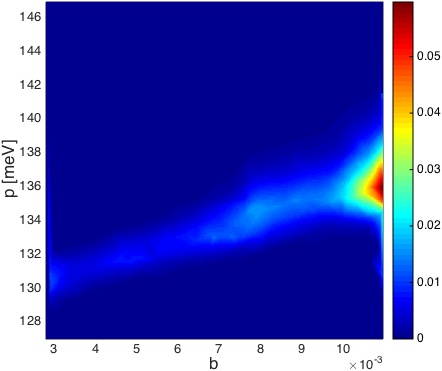
\includegraphics[width=0.7\textwidth]{NSE15-48R1_Figure13.jpg}
    %\includegraphics[width=0.45\textwidth]{srholam.eps}
    \caption[]{\label{fg:bmarscal}Calibration with BMARS.}% Only the ``Figure" label and figure number are bold.}
  \end{center}
\end{figure}

\subsection{Discussions on emulation based and direct calibrations}
{Both GPR (Figure\ \ref{fg:gprcal})\ and BMARS (Figure\ \ref{fg:bmarscal}) emulators achieve the goals set forth above. Both emulators fill give scores $b-p$ pairs without the data gaps as shown in the direct calibration results in Figure\ \ref{fg:narrow3}. In spite of the satisfactory results from the emulators,  the attendant computational cost increase due to constructing and running the emulator is almost trivial (within one hour on a single PC). This compares to the tremendous increase of cost if more MCNP simulations were needed to increase the parameter sample size.}

\section{Tests for emulation calibrated parameters}
\subsection{Calibrated parameter samplings}
Although the projections of the scores onto the main-parameter plane show similar spatial shapes, it is still critical to test if the calibrated parameter distributions {will result in robust calibrations to surrogate experiments through the process of data generation and simulation.}
All of these calibration strategies, including the direct calibration, indicate a branching ratio around $0.01$.~However, the phonon spectrum of H in \zh~used in ENDF, which is suggested by Slaggie, indicate a value of $1/241 \approx 0.00415$ \cite{Slaggie}.

For the  purpose of testing the performance of high-score parameter subsets, {28  samples were drawn from} the calibrated distributions. A rejection sampling technique was applied over the two main parameters according to the score distribution. Meanwhile, we sample uniformly over the other five parameters with LHS. Then following Step~1 through 4, MCNP generates simulation results. Figure~\ref{fg:gpsam}~and ~\ref{fg:bmsam}~show the comparisons of the sampling ranges of the main parameters before and after calibration based on GPR and BMARS, respectively. One observation is that the samples from the calibrated parameters from each emulators sharply shrink the sampling ranges, as expected. 

\begin{figure}[ht!]
\begin{subfigure}{0.5\textwidth}
\centering
\hspace*{-2.2cm}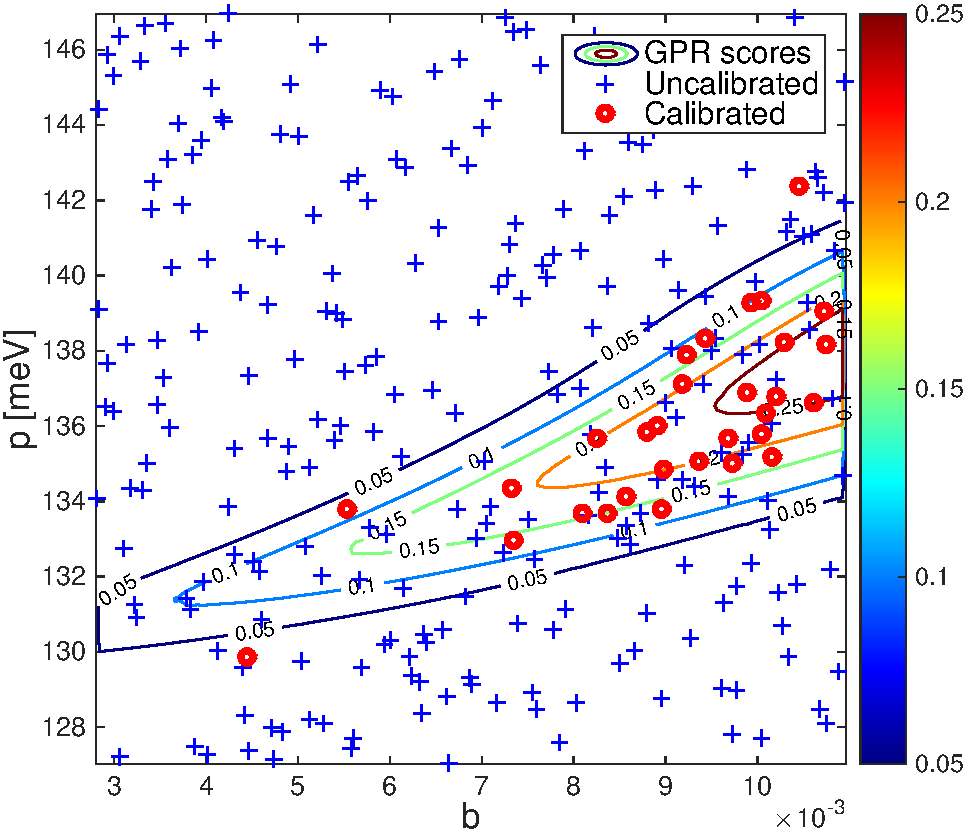
\includegraphics[width=1.4\linewidth]{NSE15-48R1_Figure14a.pdf}
\caption{Sampling over main parameters before calibration and after calibration (GPR based)}
\label{fg:gpsam}
\end{subfigure}
~
\begin{subfigure}{0.5\textwidth}
\centering
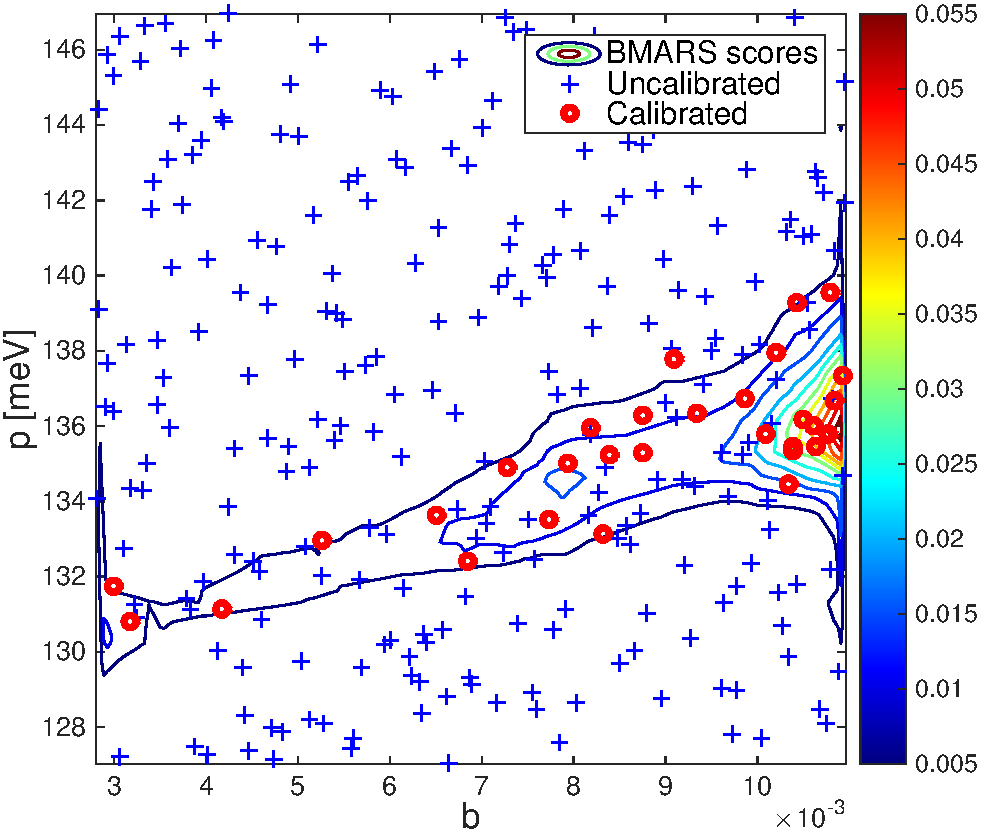
\includegraphics[width=1.45\linewidth]{NSE15-48R1_Figure14b.pdf}
\caption{Sampling over main parameters before calibration and after calibration (BMARS based).}
\label{fg:bmsam}
\end{subfigure}
\caption{Sampling of main parameters based on different emulators.}
\label{fg:testssam}
\end{figure}

\subsection{MCNP posteriori tests for calibrations}

\begin{figure}[ht!]
\begin{subfigure}{0.5\textwidth}
\centering
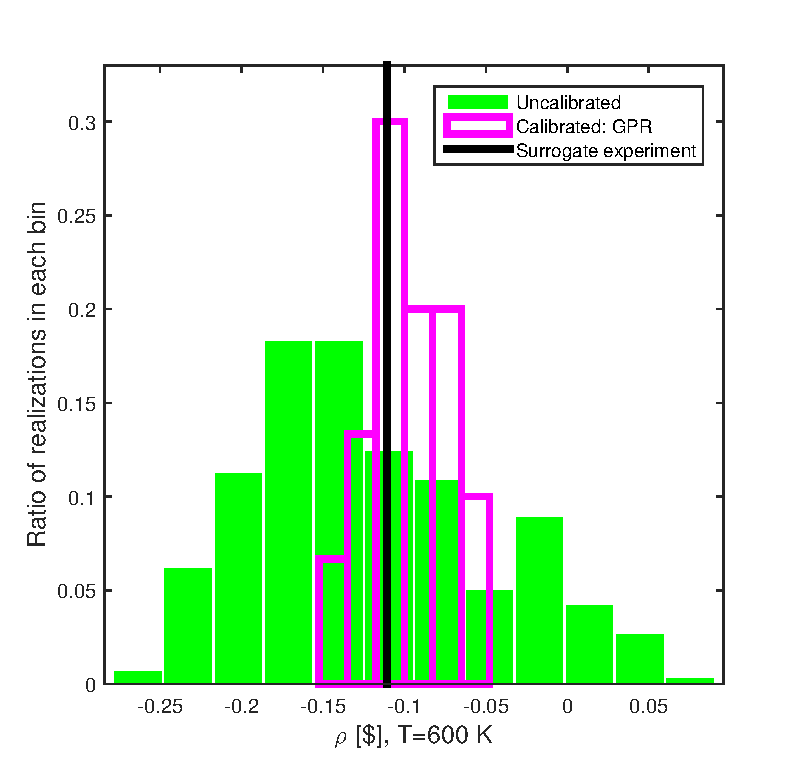
\includegraphics[width=0.9\linewidth]{NSE15-48R1_Figure15a.pdf}
%\caption{Sampling over main parameters before calibration and after calibration (BMARS based).}
\label{gptrho6k}
\end{subfigure}
~
\begin{subfigure}{0.5\textwidth}
\centering
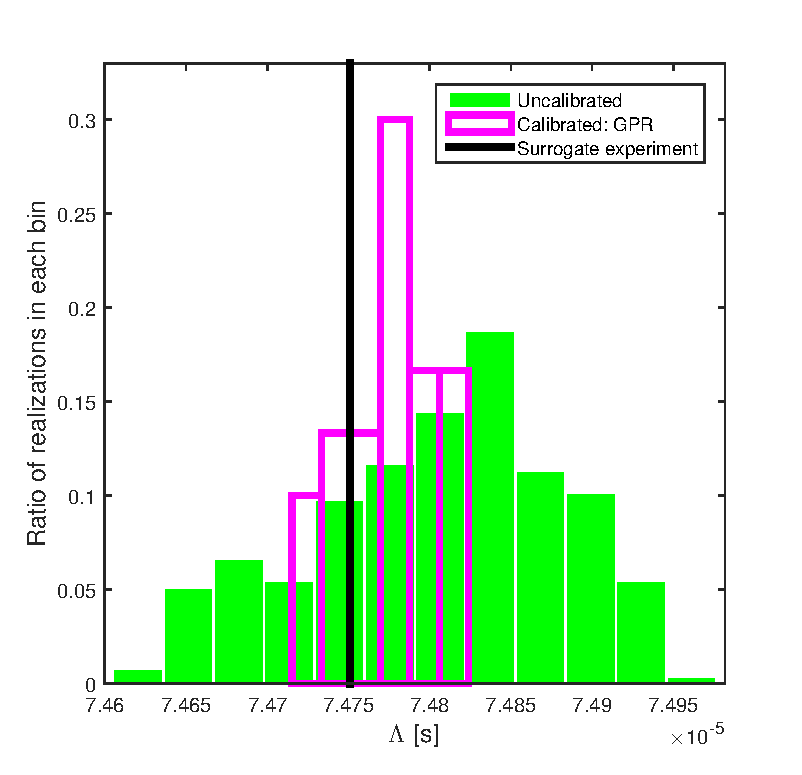
\includegraphics[width=0.9\linewidth]{NSE15-48R1_Figure15b.pdf}
%\caption{Sampling over main parameters before calibration and after calibration (GPR based)}
\label{gptlam}
\end{subfigure}
~
\begin{subfigure}{0.5\textwidth}
\centering
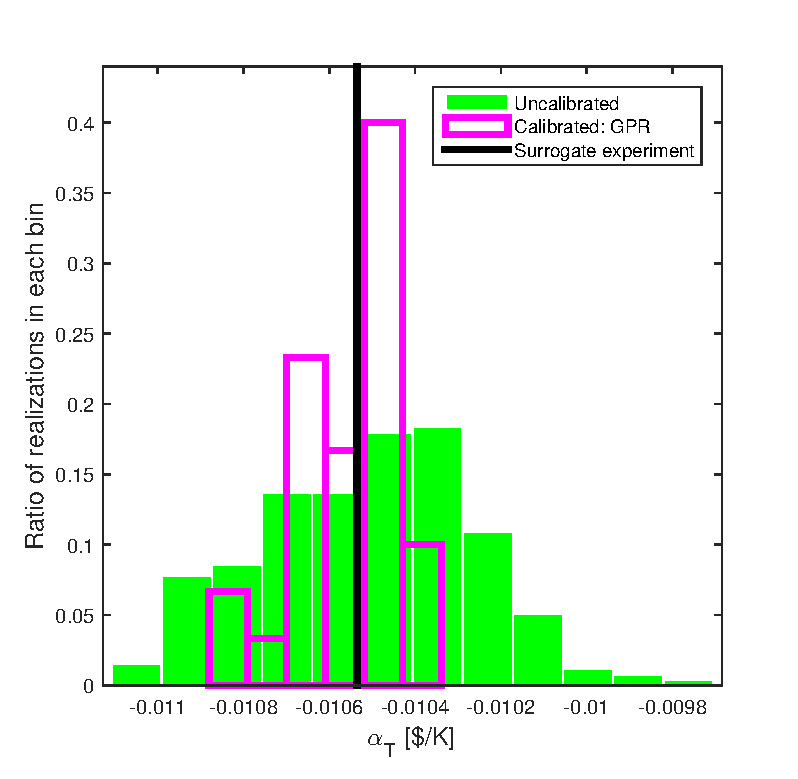
\includegraphics[width=0.9\linewidth]{NSE15-48R1_Figure15c.pdf}
%\caption{Sampling over main parameters before calibration and after calibration (BMARS based).}
\label{gpalp}
\end{subfigure}
\caption{MCNP tests for GPR based calibrations.}
\label{ttgpr}
\end{figure}

{MCNP tests with GPR- and BMARS-calibrated parameters are shown in Figure\ \ref{ttgpr}\ and \ref{ttbmars},\ respectively. Overall, calibration processes shrink uncertainties of three QoIs to different extent while surrounding the surrogate experimental results. Furthermore, though the GPR- and BMARS-based calibration process are carried out by different emulators, the calibrated parameters present comparable calibrated distributions of the QoIs.} These results are tabulated in Table \ref{tabre}.~Ranges of the mean QoI shrink. As do the standard deviations of the QoI means, e.g.~the standard deviation of reactivity at room temperature shrinks from $0.13716$~\$\ to around $0.03$~\$\ with both emulators.

A more practical question is: what if we can only afford one case to run for testing the calibration. This would be close to the real scenario for  a full-scale system. This fact motivated us to check if the calibrated parameter set with the highest-score is accurate. Fortunately, as shown in Table~\ref{tabre2},~both the BMARS based and GPR based test results, which are named ``Highest-score sample", stay within one or two standard deviations of the surrogate experimental values.


\begin{figure}[ht!]
\begin{subfigure}{0.5\textwidth}
\centering
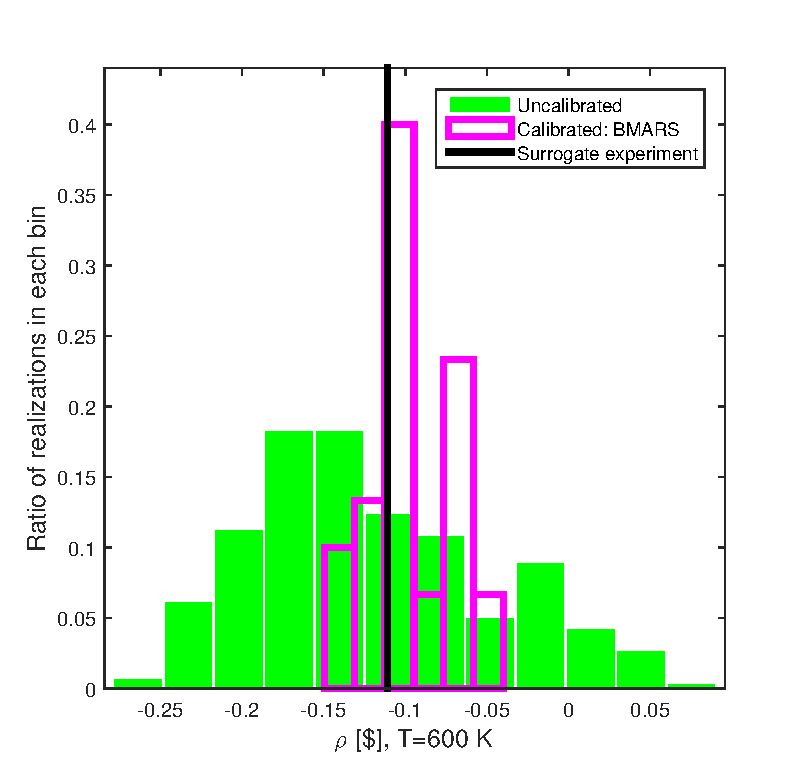
\includegraphics[width=0.9\linewidth]{NSE15-48R1_Figure16a.pdf}
%\caption{Sampling over main parameters before calibration and after calibration (BMARS based).}
\label{bmtrho6k}
\end{subfigure}
~
\begin{subfigure}{0.5\textwidth}
\centering
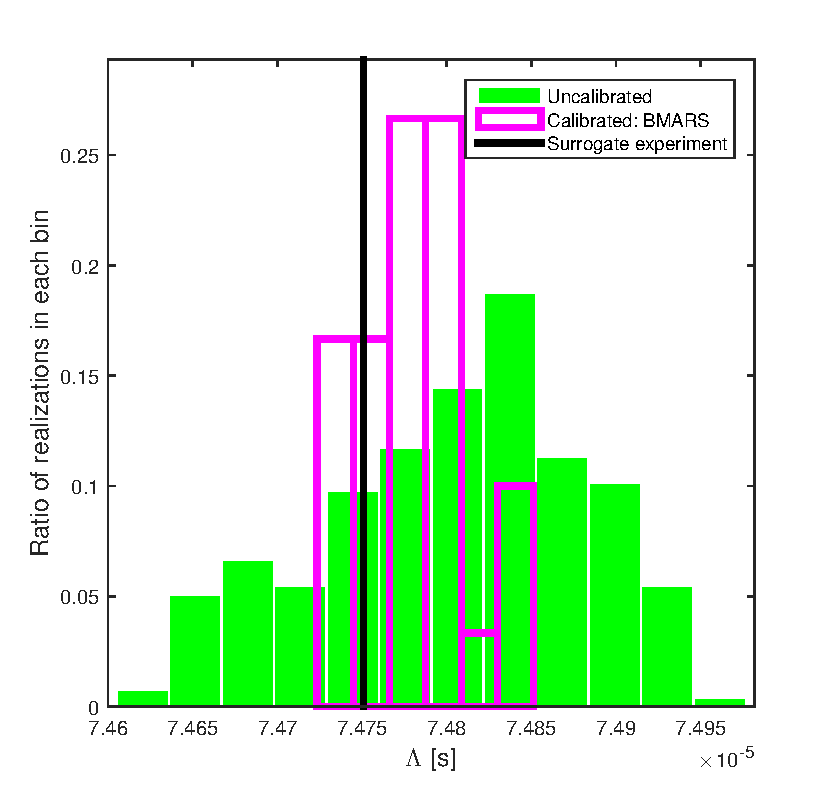
\includegraphics[width=0.9\linewidth]{NSE15-48R1_Figure16b.pdf}
%\caption{Sampling over main parameters before calibration and after calibration (GPR based)}
\label{bmlam}
\end{subfigure}
~
\begin{subfigure}{0.5\textwidth}
\centering
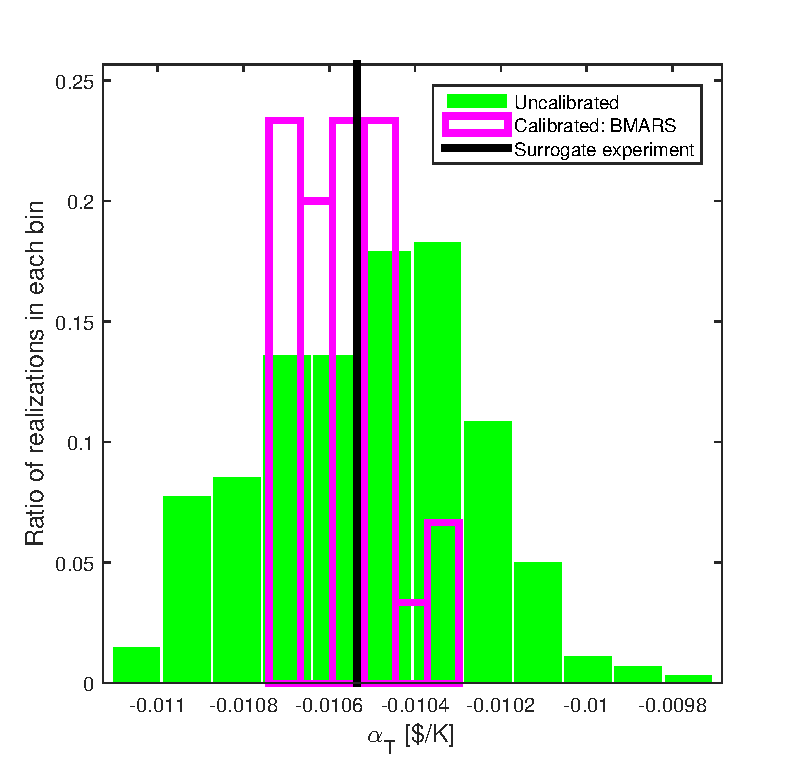
\includegraphics[width=0.9\linewidth]{NSE15-48R1_Figure16c.pdf}
%\caption{Sampling over main parameters before calibration and after calibration (BMARS based).}
\label{bmalp}
\end{subfigure}
\caption{MCNP tests for BMARS based calibrations.}
\label{ttbmars}
\end{figure}

\begin{table}
	\centering
	\caption{Reference, uncalibrated and calibrated results comparison}
%	\begin{subtable}[h]{.48\textwidth}
		\centering
		\hspace*{-1.5cm}
		\begin{tabular}{|cc|c|c|}
		\cline{1-4}
		& & $\alpha_\mathrm{T}$~[\$/K] & $\Lambda$~[s]\\
		\cline{1-4}
		\multicolumn{1}{|c|}{\multirow{4}{*}{Mean (Std.)}} & Surrogate experiments & $-0.01054~(0.00008)$ & $7.47508~(0.00194)\e{-5}$\\
		\cline{2-4}
		& \multicolumn{1}{|c|}{Uncalibrated} & $-0.01051~(0.00025)$ & $7.48043~(0.00770)\e{-5}$\\
		\cline{2-4}
		& \multicolumn{1}{|c|}{GPR calibrated}& $-0.01055~(0.00010)$& $7.47738~(0.00353)\e{-5}$\\
		\cline{2-4}
		& \multicolumn{1}{|c|}{BMARS calibrated}& $-0.01057 (0.00012)$& $7.47808~(0.00322)\e{-5}$\\
		\cline{1-4}
		\multicolumn{1}{|c|}{\multirow{3}{*}{Nominal range}} & Uncalibrated & $-0.01111\sim -0.00970$ &$7.46060\sim 7.49767\e{-5}$\\
		\cline{2-4}
		& \multicolumn{1}{|c|}{GPR calibrated}& $-0.01088\sim -0.01034$ & $7.47151\sim 7.48241\e{-5}$\\
		\cline{2-4}
		& \multicolumn{1}{|c|}{BMARS calibrated}& $-0.01074\sim -0.01030$ & $7.47234\sim 7.48511\e{-5}$\\
		\cline{1-4}
		& & $\rho_{600\mathrm{K}}$~[\$] & \multicolumn{1}{|c|}{\multirow{7}{*}{}}\\
		\cline{1-3}
		\multicolumn{1}{|c|}{\multirow{4}{*}{Mean (Std.)}} & Surrogate experiments & $-0.11085~(0.01695)$&\\
		\cline{2-3}
		& \multicolumn{1}{|c|}{Uncalibrated} & $-0.12151~(0.07266)$&\\
				\cline{2-3}
		& \multicolumn{1}{|c|}{GPR calibrated}& $-0.09612~(0.02679)$&\\
		\cline{2-3}
		& \multicolumn{1}{|c|}{BMARS calibrated}& $-0.09493~(0.02667)$&\\
		\cline{1-3}
		\multicolumn{1}{|c|}{\multirow{3}{*}{Nominal range}} & Uncalibrated & $-0.27897\sim 0.09072$&\\
		\cline{2-3}
		& \multicolumn{1}{|c|}{GPR calibrated}& $-0.15246\sim -0.04771$&\\
		\cline{2-3}
		& \multicolumn{1}{|c|}{BMARS calibrated}& $-0.14938\sim -0.04001$&\\
		\cline{1-4}
		\end{tabular}
		
%	\end{subtable}


	\label{tabre}
\end{table}


\begin{table}
	\centering
	\caption{Reference, uncalibrated and highest-score sample comparisons}
%	\begin{subtable}[h]{.48\textwidth}
		\centering
		\hspace*{-1.5cm}
		\begin{tabular}{|cc|c|c|}
		\cline{1-4}
		\multicolumn{2}{|c|}{QoIs}& $\alpha_\mathrm{T}$~[\$/K] & $\Lambda$~[s]\\
		\cline{1-4}
		\multicolumn{1}{|c|}{\multirow{1}{*}{Mean (Std.)}} & Surrogate experiments & $-0.01054~(0.00008)$ & $7.47508~(0.00194)\e{-5}$\\
		\cline{1-4}
		\multicolumn{1}{|c|}{\multirow{2}{*}{Highest-score Sample (Std.)}} & GPR calibrated & $-0.01051~(0.00007)$ & $7.47729~(0.00194)\e{-5}$\\
		\cline{2-4}
		& \multicolumn{1}{|c|}{BMARS calibrated} & $-0.01062~(0.00007)$ & $7.48013~(0.00202)\e{-5}$\\
		\cline{1-4}
		\multicolumn{1}{|c|}{\multirow{1}{*}{Nominal range}} & Uncalibrated & $-0.01111\sim -0.00970$ &$7.46060\sim 7.49767\e{-5}$\\
		\cline{1-4}
		\multicolumn{2}{|c|}{QoIs}& $\rho_{600\mathrm{K}}$~[\$] & \multicolumn{1}{|c|}{\multirow{5}{*}{}}\\
		\cline{1-3}
		\multicolumn{1}{|c|}{\multirow{1}{*}{Mean (Std.)}} & Surrogate experiments  & $-0.11085~(0.01695)$ &\\
		\cline{1-3}
		\multicolumn{1}{|c|}{\multirow{2}{*}{Highest-score Sample (Std.)}} & GPR calibrated  & $-0.09852~(0.01540)$ &\\
		\cline{2-3}
		& \multicolumn{1}{|c|}{BMARS calibrated} & $-0.10161~(0.01695)$&\\
		\cline{1-3}
		\multicolumn{1}{|c|}{\multirow{1}{*}{Nominal range}} & Uncalibrated &  $-0.27897\sim 0.09072$&\\
		\cline{1-4}
		\end{tabular}
		
%	\end{subtable}

	\label{tabre2}
\end{table}

\subsection{Extrapolated test}
We calibrated the PPS parameters with $\rho_{600\mathrm{K}}$,\ $\alpha_T$~and $\Lambda_{600\mathrm{K}}$. Since the scattering data for the surrogate experiment is from ENDF, which is based upon using a single phonon spectrum for all temperatures\cite{NJOY}, it is reasonable to hypothesize that the thermal scattering data with calibrated PPS model parameters, which means the same phonon spectrum, at 600~K shall result in accurate simulation posterior distributions for QoIs at 293.6~K as well. Figure~\ref{exp}~presents the reactivity at 293.6~K simulated with data before calibration and after calibration. The uncertainties of both results decrease as expected. Corresponding results are tabulated in Table~\ref{exptab}.

\begin{figure}[ht!]
\begin{subfigure}{0.5\textwidth}
\centering
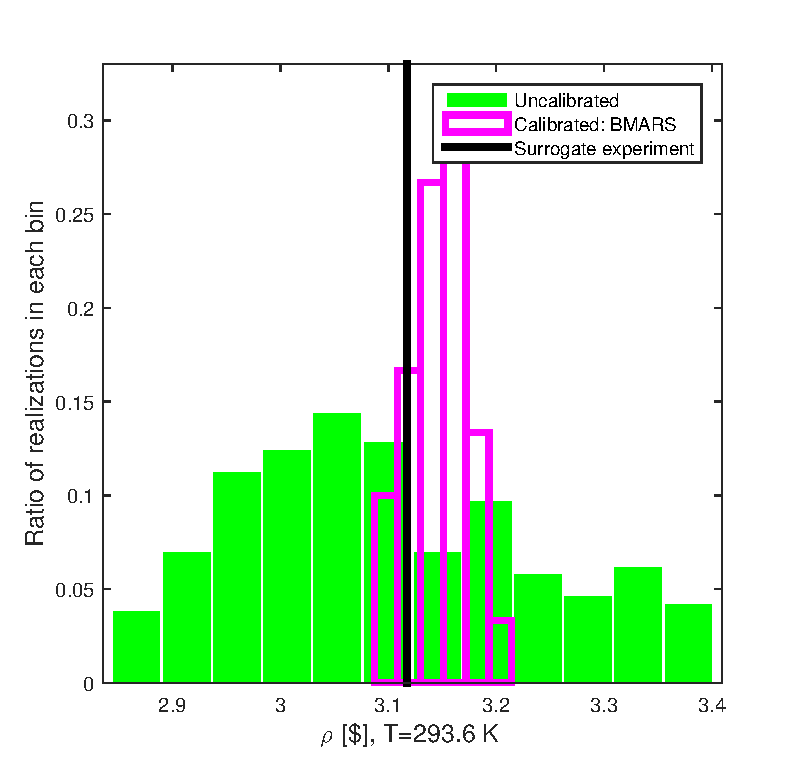
\includegraphics[width=0.9\linewidth]{NSE15-48R1_Figure17a.pdf}
%\caption{}
%\label{bmtrhort}
\end{subfigure}
~
\begin{subfigure}{0.5\textwidth}
\centering
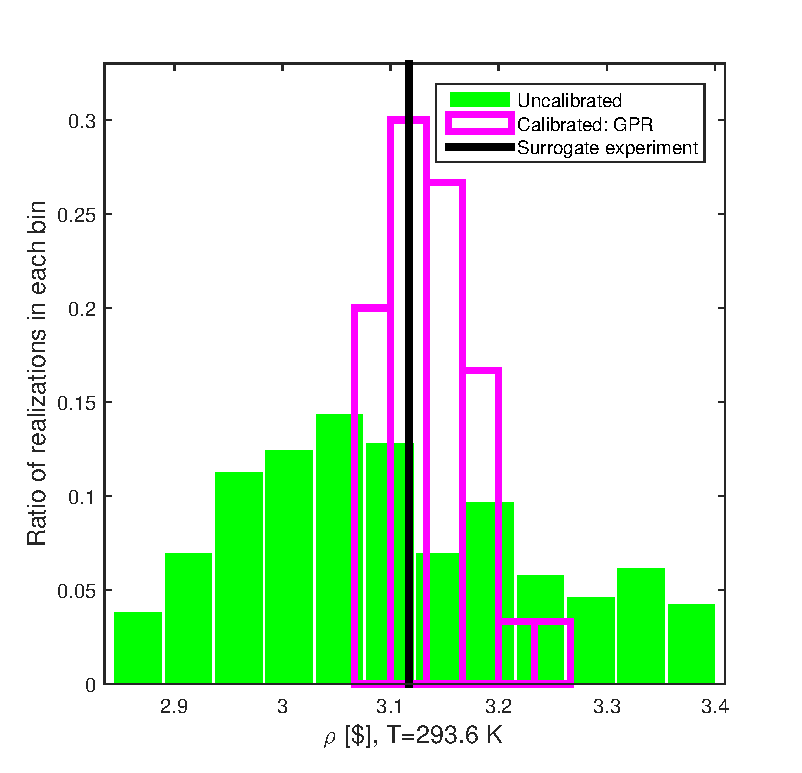
\includegraphics[width=0.9\linewidth]{NSE15-48R1_Figure17b.pdf}
%\caption{}
%\label{gptrhort}
\end{subfigure}
\caption{Extrapolation tests for $\rho$~at $T=293.6$~K using calibrated parameters from QoIs calibrated at $600$~K.}
\label{exp}
\end{figure}

\begin{table}
	\centering
	\caption{Reference, uncalibrated and highest-score sample comparisons}
%	\begin{subtable}[h]{.48\textwidth}
		\centering
		\hspace*{-1.5cm}
		\begin{tabular}{|cc|c|}
		\cline{1-3}
		\multicolumn{2}{|c|}{QoI}& $\rho_{293.6\mathrm{K}}$~[\$]\\
		\cline{1-3}
		\multicolumn{1}{|c|}{\multirow{1}{*}{Mean (Std.)}} & Surrogate experiments & $3.11708~(0.01658)$\\
		\cline{1-3}
		\multicolumn{1}{|c|}{\multirow{2}{*}{Highest-score Sample (Std.)}} & GPR calibrated & $3.12151~(0.01477)$\\
		\cline{2-3}
		& \multicolumn{1}{|c|}{BMARS calibrated} & $3.15399~(0.01476)$\\
		\cline{1-3}
		\multicolumn{1}{|c|}{\multirow{3}{*}{Nominal range }} & Uncalibrated & $2.84338\sim 3.40155$\\
		\cline{2-3}
		& \multicolumn{1}{|c|}{GPR calibrated}& $3.06685\sim 3.26608$\\
		\cline{2-3}
		& \multicolumn{1}{|c|}{BMARS calibrated}& $3.08754\sim 3.21448$\\
		\cline{1-3}
		\end{tabular}
		
%	\end{subtable}


	\label{exptab}
\end{table}

\section{Concluding remarks}
\subsection{Summary}
Previously, we established a seven-parameter phonon spectrum model for \zh~in TRIGA reactor. Based on this model, we sampled the parameters, generated thermal scattering data of \zh\ and performed criticality simulations. Also, we used TRIGA reactor simulations as a surrogate experiment. In the process, we developed scoring algorithm to estimate the similarities between the simulations and the surrogate experiment. Then a calibration framework for the parameters of the parameterized phonon spectrum models based on the scores was established.

In this work, we extended the calibration framework. Instead of estimating the scores using simulation results, we invoked emulators, in particular  Gaussian process regression and Bayesian multivariate adaptive regression splines, to emulate the mapping from the proposed parameters to the QoIs. Scoring is performed based upon estimating similarities of the surrogate experiment and emulation results at designated input parameter points. When projecting the scores into parameter space, it is noticed that both emulators narrowed the preferred parameter sets down. Posteriori criticality test results with parameters sampled based on the scores resulted from both emulators illustrate the effectiveness of the extension of the calibration framework. Uncertainties of the QoIs narrow down to different extent, e.g.~the range of mean values of $\rho_{600\mathrm{K}}$~change from $[-0.27897,0.09072]$~\$\ to $-0.14938\sim -0.04001$\ \$ (BMARS based) and $-0.15246\sim -0.04771$~\$ (GPR based).

We also extended the posteriori test with the thermal scattering data produced with the same phonon spectra used in 600~K to room temperature (293.6~K) as an example of an extrapolation experiment. We found the the using the parameter ranges calibrated at 600 K  were still accurate at room temperature.

{Though the emulation based framework accomplished the aforementioned goal, there remain uncertainties in the simulations used in our calibrations. The MCNP simulations were carried out with large numbers of particles such that the statistical error of each simulation QoI is much smaller than the total variations of QoIs. In such a case, the mean values of QoIs are used as the input of the emulators to emulate the mapping from input to output without affecting the calibration accuracy. Nonetheless, this would not be true when the uncertainties of simulation QoIs are not negligible. In such a case, using the nominal means of simulation QoIs as emulation inputs would introduce noticeable statistical errors. In such a case we would need to account for the uncertainty in the simulation results.}

\tcb{Though the calibration framework developed here is based on \zh\ in a TRIGA reactor, the methodology is not limited to that system. We believe that the framework could also be applied to the materials with thermal scattering, e.g.,\ water, in light water reactors (LWRs).}

\subsection{Future work}
We investigated three types of sensitive QoIs in this work at 600~K. To further constrain the calibration, more sensitive QoIs are needed. We previously investigated the total absorption rates over the whole energy range of ex/in-core neutron detectors and claimed the insensitivity of such QoIs to the phonon spectrum \cite{physor}. Yet, recent, more detailed simulations indicate that detectors measuring only the thermal flux will be sensitive to our parameters. This observation should not be a surprise since when we manipulate the phonon spectrum, the thermal scattering cross sections are changed, which results in the variation of the up-scattering and thus the thermal flux\cite{thesis,weixiong}. We believe monitoring the thermal absorption rate with detectors could bring in another constraint besides the ones used in this paper. Such in-core thermal neutron detectors will be available soon in the Texas A\&M TRIGA reactor.

%The surrogate experiment, which is the criticality simulation with ENDF-VII data, is produced with a unique phonon spectrum at all temperatures, which justify our extrapolation test at 293.6~K with parameterized phonon spectrum calibrated at 600~K. Yet, in practice, phonon spectra vary when temperature changes\cite{Badea,Harling},~which indicates calibrations at different temperatures are supposed to be carried out individually with realistic experimental data.

Also, the temporal impact of varying phonon spectrum of \zh~in applications such as pulse experiments should be investigated and corresponding calibration work should be done for TRIGA reactors.




\section*{Acknowledgments}
This project is funded by Department of Energy NEUP research grant from Battelle Energy Alliance, LLC- Idaho National Laboratory, Contract No: C12-00281. The authors would like to thank the anonymous reviewers of this work for their thoughtful comments that served to make this a stronger paper.
\section*{References}

\bibliography{NSE15-48R1_LaTeX_bibliography}

\end{document}